\part{Contribution}

\chapter{Conception}

%\newpage

\section{Introduction}
Le domaine de l'apprentissage profond a connu une grande croissance de la profondeur des architectures de réseaux de neurones. Cependant, cette croissante pose des défis importants en termes d'exigences de calcul et mémoire et de consommation d'énergie. Ainsi, la nécessité de concevoir des techniques efficaces de compression et d'optimisation des modèles est devenue primordiale. Dans ce chapitre, nous présenterons une méthode automatique pour l'elagage des réseaux neuronaux très profonds qui exploite l'apprentissage par renforcement et le plongement des couches du réseau.

\section{Vue globale de la solution}
L'élagage des réseaux de neurones profonds est devenu une technique essentielle afin de déployer ces réseaux sur des appareils mobiles disposant de ressources de calcul et de stockage limitées. Plusieurs techniques existent pour élaguer un réseau. Cependant, ces techniques nécessitent des experts du domaine afin d'explorer le vaste espace de conception et obtenir un bon compromis entre la taille, la vitesse et la précision du modèle, ce qui peut prendre beaucoup de temps et ne produit pas toujours des résultats optimals.

Dans cette partie, nous proposons une nouvelle méthode d'élagage automatique des réseaux de neurones profonds qui utilise l'apprentissage par renforcement et les technique de plongement pour fournir les pourcentages d'élagage optimals. Notre méthode, contrairement aux méthodes conventionnelles, ne nécessite pas d'experts humains dans le domaine et prend moins de temps.

Dans les réseaux de neurones profonds, les couches ne sont pas indépendantes les unes des autres en raison de la manière dont l'information est propagée et traitée à travers le réseau. Chaque couche prend les sorties de la couche précédente en entrée et génère des sorties qui sont ensuite utilisées comme entrées pour la couche suivante. Cette interconnexion crée des relations et des dépendances entre les couches.

Lors de l'apprentissage, les poids et les biais de chaque couche sont ajustés et chaque couche contribue de manière spécifique à la transformation des données en fonction des poids et des biais. Donc, les ajustements dans une couche peuvent avoir un impact sur les performances et les caractéristiques apprises par les autres couches, et cela affecte directement la précision de notre modèle. Pour cela, nous avons décider d'utiliser une stratégie d'élagage continue. Nous commençons par l'initialisation des paramètres de notre modèle avec des valeurs aléatoires et puis nous entraînons le modèle jusqu’à l'obtention d'une bonne précision. Ensuite, nous commençons le processus d'élagage où nous utilisons un agent DDPG pour élaguer le réseau couche par couche (comme illustrée dans la figure \ref{fig:global-solution}). Pour chaque couche $L_n$ , l'agent DDPG reçoit comme entrée le plongement de la couche qui permet de préserver les caractéristiques utiles de cette couche, puis il génère en sortie un taux d'élagage $a_n$. Après l'élagage de la couche $L_n$ avec le taux $a_n$, l'agent DDPG passe à la couche suivante $L_{n+1}$.

\begin{figure}[hbt!]
  \centering
  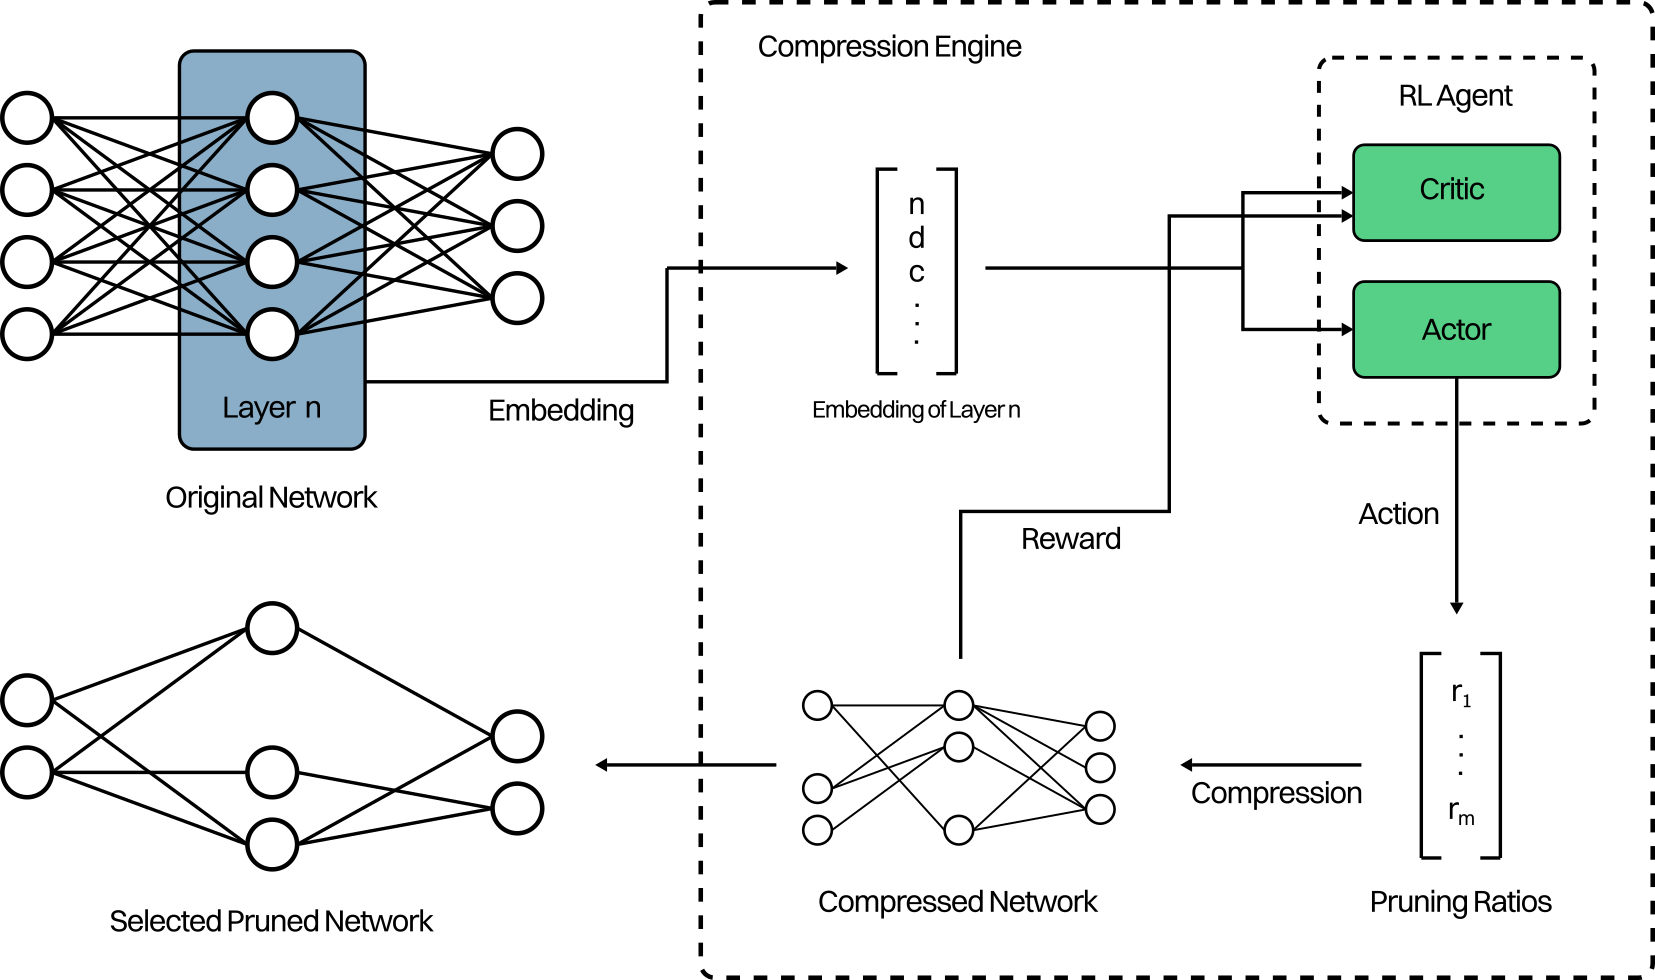
\includegraphics[width=14cm]{images_pfe/global-solution.png}
  \caption{Présentation du processus d'élagage.}
  \label{fig:global-solution}
\end{figure}
\FloatBarrier
\medskip


Une fois toutes les couches élaguées, nous évaluons la précision du modèle sans réglage fin afin d'estimer la précision du modèle final (avec le réglage fin). Cette valeur approchée permet d'améliorer le temps de recherche sans avoir à ré-entraîner le modèle à chaque fois. Une fois la recherche terminée, nous effectuons un réglage fin au modèle avec la meilleure précision pour améliorer encore sa précision.

Généralement, nous pouvons décomposer le processus d'élagage en 4 étapes principales (comme illustré dans la figure \ref{fig:global-schema}):
\begin{enumerate}
    \item \textbf{Initialisation}: Nous commençons par le définition du modèle et l'initialisation aléatoire de ses paramètres.
    \item \textbf{Entraînement}: Nous entraînons le modèle à l'aide du jeu de données CIFAR-10 jusqu'à ce que nous obtenions la meilleure précision.
    \item \textbf{Élagage}: Nous utilisons l'agent DDPG pour fournir les pourcentages d'élagage de chaque couche, et nous sélectionnons le meilleure réseau parmi les réseaux élagués pour l'améliorer dans l'étape suivante.
    \item \textbf{Réglage fin}: Nous ré-entraînons le réseau obtenu dans l'étape précédente pour améliorer encore sa précision.
\end{enumerate}

\begin{figure}[hbt!]
  \centering
  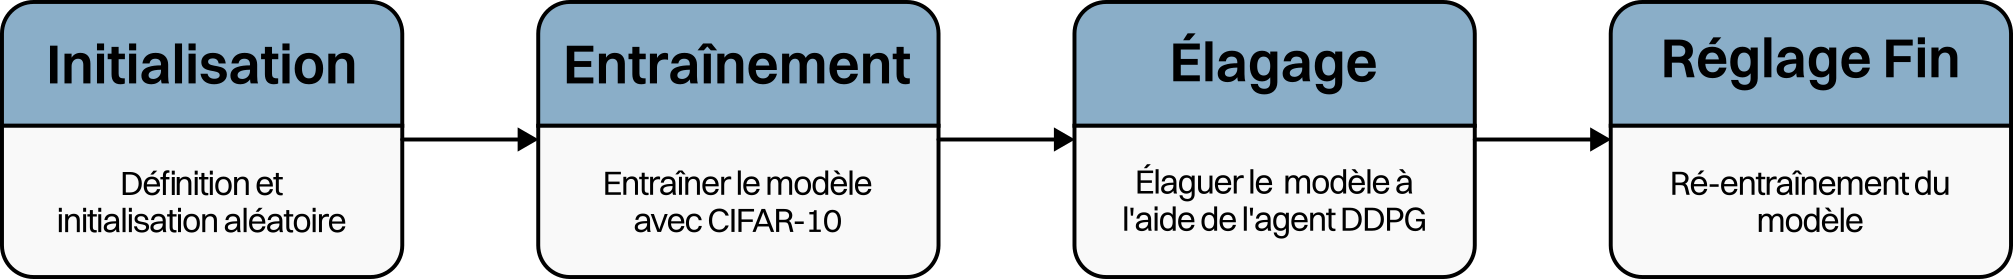
\includegraphics[width=14cm]{images_pfe/schema-general.png}
  \caption{Schéma global du processus d'élagage.}
  \label{fig:global-schema}
\end{figure}
\FloatBarrier
\medskip

\section{Plongements des couches}
Il existe plusieurs architectures de réseaux de neurones et les couches et les connexions entre elles diffèrent d’une architecture à l’autre. Dans ce travail, nous allons concentrer uniquement sur les réseaux de neurones de convolution et résiduels, qui utilisent deux types de couches seulement: les couches de convolution et les couches entièrement connectées.

Comme illustrée dans la figure \ref{fig:global-solution}, l'agent DDPG reçoit le plongement de la couche $L_n$ en entrée et fournit en sortie le taux d'élagage $a_n$ de cette couche. La raison derrière l'utilisation du plongement de couche au lieu du plongement d'un graphe de calcul avec encodeur GCN (qui est utilisé dans la méthode de \cite{pfe2022}) est que le plongement de couche est généralement plus simple à mettre en œuvre et plus rapide.

D'une part, le plongement de couche peut simplifier la représentation d'entrée et réduire la dimensionnalité par rapport à une représentation graphique, ce qui rend les données plus faciles à traiter et l'apprentissage plus rapide. D'autre part, lors de l'utilisation du graphe de calcul avec GCN, la construction et reconstruction du graphe entraînent une surcharge à chaque étape de l'apprentissage par renforcement. Nous devons toujours reconstruire le graphe de calcul en fonction du taux d'élagage actuel, ce qui peut être coûteux en termes de calculs et peut ralentir le processus d'élagage, tandis que dans les plongements de couches, nous trouvons qu'ils sont plus interprétables et nécessitent moins d'efforts pour les construire, visualiser et comprendre par rapport aux structures graphiques. Finalement, la complexité des méthodes basées sur GCN peut augmenter considérablement lorsque la taille du réseau de neurones augmente, ce qui n'est pas le cas pour les plongement de couches car ils sont plus évolutives et fonctionnent mieux dans des environnements à grande échelle.

Chaque plongemenet $s_n$ est caractérisé par 11 caractéristiques qui sont essentielles pour que l’agent DDPG puisse distinguer une couche d’une autre. Ces caractéristiques sont les suivantes:
\begin{equation}
    (n, d, c, h, w, stride, k, FLOPs[n], removed, remaining, a_{n−1} )
\end{equation}
où:
\begin{conditions}
    n & L'indice de la couche\\
    d et c & Les canaux de sortie et d'entrée\\
    h & Le nombre de pixels dans la direction verticale\\
    w & Le nombre de pixels dans la direction horizontale\\
    stride & La taille du pas du filtre\\
    k & La taille du noyau\\
    FLOPs[n] & Les FLOPs de la couche $L_n$\\
    removed & Le nombre total de FLOPs supprimés dans les couches précédentes\\
    remaining & Le nombre de FLOPs restants dans les couches suivantes\\
    a_{n-1} & Le taux d'élagage de la couche précédente\\
\end{conditions}
% \begin{itemize}
%     \item \textit{n}: L'indice de la couche
%     \item \textit{d} et \textit{c}: Les canaux de sortie et d'entrée
%     \item \textit{h}: Le nombre de pixels dans la direction verticale
%     \item \textit{w}: Le nombre de pixels dans la direction horizontale
%     \item \textit{stride}: La taille du pas du filtre
%     \item \textit{k}: La taille du noyau
%     \item \textit{FLOPs[n]}: Les FLOPs de la couche $L_n$
%     \item \textit{removed}: Le nombre total de FLOPs supprimés dans les couches précédentes
%     \item \textit{remaining}: Le nombre de FLOPs restants dans les couches suivantes
%     \item $a_{n-1}$: Le taux d'élagage de la couche précédente
% \end{itemize}

Après l'extraction de ces caractéristiques, nous effectuons une normalisation afin de les préparer à être utilisées comme entrées dans l'agent DDPG. La normalisation garantit que les valeurs des caractéristiques extraites se situent dans une plage similaire. Ceci est important pour la stabilité de l'entraînement et la convergence de l’agent DDPG. Il existe plusieurs méthodes pour faire la normalisation telles que:
\begin{itemize}
    \item \textbf{Min-Max scaling}: Cette méthode transforme les valeurs des caractéristiques en une plage prédéfinie, souvent [0, 1] ou [-1, 1]. Il faut d'abord Identifier les valeurs minimales et maximales de la caractéristique, puis soustrayez la valeur minimale et divisez par la plage (maximum moins minimum) pour chaque valeur de la caractéristique.
    \item \textbf{Z-Score (standardisation)}: Cette méthode met à l'échelle les valeurs pour avoir une moyenne de 0 et un écart type de 1. D'abord, on calcule la moyenne et l’écart type de la caractéristique. Puis, pour chaque valeur de la caractéristique, on soustrait la moyenne et on divise par l'écart type.
    \item \textbf{Feature Scaling}: Avec cette méthode, on met à l'échelle chaque caractéristique individuellement pour avoir une moyenne de 0 et une variance de 1. Ceci peut être réalisé en soustrayant la moyenne et en divisant par l'écart type pour chaque caractéristique séparément.
\end{itemize}

Dans notre cas, nous allons utiliser la méthode Min-Max scaling pour garantir que toutes les valeurs sont ajustées proportionnellement pour s'adapter à la plage [0, 1].

\section{Choix des pourcentages d'élagage}
Afin de choisir les meilleurs pourcentages d'élagage, nous disposons de certaines métriques qui guident ce processus. Ces métriques sont essentielles pour l'évaluation des performances des réseaux de neurones élagués. Les métriques que nous examinerons comprennent le temps d'inférence et la taille du réseau.

Le temps d'inférence est une mesure du délai nécessaire pour obtenir une sortie suite à la présentation d'une entrée au réseau, c'est à dire c'est le temps nécessaire pour faire une propagation vers l'avant. Une diminution de ce temps se traduit par une amélioration de la réactivité globale du réseau. De plus, la réduction de la taille du réseau apporte plus d'avantages, allant de la réduction des besoins en espace de stockage à une consommation énergétique réduite.

Cependant, ces deux métriques sont liées à un paramètre important: le degré de sparsité du réseau, qui, lorsqu'il augmente, il peut engendrer des gains significatifs en termes de taille du réseau et de rapidité d'inférence. Ce paramètre mesure la proportion de paramètres qui ont été élagués par rapport au nombre total de paramètres dans le modèle d'origine. Toutefois, nous pouvons avoir une perte de performances du modèle lorsque nous augmentons extrêmement le degré de sparsité du réseau. Il est donc nécessaire de trouver un équilibre entre la réduction de la taille et le maintien des performances.

Pour augmenter le degré de sparsité du réseau, nous devons réduire/augmenter l'une des 4 mesures suivantes: les paramètres du réseau, les FLOPs, les FLOPS, ou les MAC.

\subsubsection{Paramètres}
Les paramètres font référence aux poids et aux biais qui sont ajustés pendant l'entraînement du réseau. Chaque connexion entre les neurones est associée à un poids, qui détermine l'importance de cette connexion pour le calcul de la sortie. En ajustant ces poids et biais lors de la phase d'entraînement, le réseau apprend à représenter les relations entre les entrées et les sorties. Le nombre total de paramètres dans un réseau est un facteur crucial qui, avec son augmentation, peut rendre le réseau plus grand en termes de taille et complexe à entraîner.

Prenons l'exemple d'un réseau de neurones convolutionnel (CNN). Chaque couche de ce réseau contient des filtres qui glissent sur l'image d'entrée pour extraire des caractéristiques. Chaque connexion entre un filtre et une région de l'image a un poids associé. Ces poids constituent les paramètres du réseau. Par exemple, si nous avons un filtre de taille 3x3, il y aura 9 poids (un pour chaque connexion) et un biais associé à ce filtre. Si le réseau a plusieurs de ces filtres dans une couche, le nombre total de paramètres augmentera en conséquence.

\subsubsection{FLOPs}
Les FLOPs (Floating Point Operations) sont une mesure du nombre total des opérations en virgule flottante effectués par le modèle, telles que les additions, les soustractions, les multiplications et les divisions. Un modèle avec un grand nombre de FLOPs peut nécessiter plus de ressources de calcul et de temps pour l'entraînement et l'inférence.

Souvent, le nombre de paramètres est utilisé pour mesurer la complexité du modèle, mais il ne se traduit pas directement en charge computationnelle lors de l'inférence. Dans ce travail, nous allons utiliser les FLOPs comme critère de choix des pourcentage d’élagage au lieu d'utiliser les paramètres. Les raisons de ce choix sont citées dans la section suivante.

\subsubsection{FLOPS}
Les FLOPS (Floating Point Operations per Second) sont le nombre d'opérations en virgule flottante qui peut être effectuer par seconde et ils sont utilisés pour évaluer la capacité de calcul et les performances d'un dispositif ou des unités de traitement, telles que les processeurs et les GPU. Plus le nombre de FLOPS est élevé, plus le dispositif est capable de réaliser des calculs complexes rapidement et l’inférence sera plus rapide.

Par exemple, pour une carte graphique (GPU) qui a une capacité de calcul de 10 téraflops ($10 \cdot 10^{12} FLOPS$), elle peut effectuer environ 10 billions d'opérations en virgule flottante par seconde. Cela serait particulièrement utile pour accélérer l'entraînement des réseaux très profonds.

\subsubsection{MAC}
Un MAC (Multiply-Accumulate Computations) combine une multiplication suivie d'une addition de produits résultants. Il est utilisé pour calculer les sorties des neurones en multipliant les entrées par les poids associés, puis en accumulant ces produits pour obtenir la sortie finale du neurone. Généralement, on considère 1 MAC = 2 FLOPs.

\subsection{Raisons d'utilisation des FLOPs}
Dans les réseaux CNN, la réduction du nombre de paramètres ne se traduit pas nécessairement par une réduction proportionnelle en termes d'opérations en virgule flottante (FLOPs). Ces dernières dépendent de plusieurs facteurs au-delà du simple nombre de paramètres, tels que:
\begin{itemize}
    \item \textbf{Taille des filtres}: La taille des filtres de convolution affecte le nombre de calculs. Les filtres plus grands nécessitent plus de calculs par couche.
    \item \textbf{Taille de l'entrée}: La taille de l'entrée d'une couche affecte également le nombre de calculs. Des dimensions d'entrée plus grandes nécessitent plus de calculs pour être traitées.
    \item \textbf{Stride}: Le stride (pas) détermine comment les filtres de convolution se déplacent à travers les données d'entrée. Les pas plus grands réduisent le nombre de calculs, car ils sautent certaines régions de l'entrée.
    \item \textbf{Pooling}: Les couches de regroupement maximal (maxpool) ou de regroupement moyen (avgpool) sont utilisées dans les CNN pour réduire les dimensions spatiales. Ces couches affectent également la charge de calcul globale.
    \item \textbf{Non-linéarité}: Les fonctions d'activation telles que ReLU introduisent des calculs supplémentaires lors des passes avant et arrière.
    \item \textbf{Connexions sautées et blocs résiduels}: Les connexions sautées ou les blocs résiduels peuvent introduire des calculs supplémentaires.
\end{itemize}

Prenons un exemple simple avec deux couches de convolution dans le réseau. Supposons que les deux couches ont le le même filtre et stride mais la première couche possède une entrée plus grande que la deuxième, c'est a dire que la deuxième couche nécessitera moins de FLOPs par rapport à la première couche. Nous avons donc deux scénarios: 
\begin{enumerate}
    \item \textbf{Élagage en pourcentage de paramètres}: Dans ce scénario, si on élague 25\% de la première couche et 75\% de la deuxième couche, on va élaguer donc 50\% des paramètres ($\frac{25+75}{2}$). Cela réduit le nombre total de paramètres, mais ne correspond pas nécessairement à une réduction proportionnelle des calculs car la première couche a plus de calculs que la deuxième couche (la réduction des FLOPs pourrait être bien inférieure à 50\%).
    \item \textbf{Élagage en pourcentage de FLOPs}: Contrairement à la réduction de paramètres, si on élague 50\% de FLOPs, alors on va élaguer 50\% des calculs, ce qui est plus avantageux.
\end{enumerate}

\subsection{Calcul des FLOPs}
Comme indiqué précédemment, le nombre des FLOPs peut être influencé par plusieurs facteurs, tels que la taille d'entrée, le stride, la taille du filtre, etc. L'estimation du nombre de FLOPs ne tient peut-être pas compte de toutes les complexités des opérations spécialisées, des optimisations matérielles et des détails d'implémentation, mais elle fournit une estimation approximative de la complexité de notre modèle.

Pour calculer le nombre des FLOPs dans un modèle, nous avons des règles différentes pour chaque type de couche:
\begin{itemize}
    \item \textbf{Couche de convolution} \begin{equation}
        FLOPs = 2 \cdot C_I \cdot C_O \cdot K \cdot O
    \end{equation}
    \item \textbf{Couche entièrement connectée} \begin{equation}
        FLOPs = 2 \cdot I \cdot O
    \end{equation}
\end{itemize}

où:
\begin{conditions}
    C_I & Le nombre de canaux d'entrée\\
    C_O & Le nombre de canaux de sortie\\
    K & La forme du noyau\\
    I & La taille de l'entrée\\
    O & La taille de la sortie\\
\end{conditions}
% \begin{itemize}
%     \item $C_I$: Le nombre de canaux d'entrée
%     \item $C_O$: Le nombre de canaux de sortie
%     \item \textit{K}: La forme du noyau
%     \item \textit{I}: La taille de l'entrée
%     \item \textit{O}: La taille de la sortie
% \end{itemize}

Supposons que nous avons le modèle suivant qui effectue une classification sur le jeu de données MNIST, où:
\begin{itemize}
    \item La taille de l'entrée est 28x28x1 (niveaux de gris)
    \item Nous commençons par 2 convolutions de 5 noyaux de taille (3x3)
    \item Nous exécutons ensuite une couche entièrement connectée de 128 neurones
    \item Nous terminons avec une couche entièrement connectée de 10 neurones
\end{itemize}

Donc, le nombre de FLOPs pour les 4 couches de notre modèle est calculé comme suit:
\begin{itemize}
    \item \textbf{Première convolution}: $2 × 1 × 5 × (3 × 3) × 26 × 26 = 60 840 FLOPs$
    \item \textbf{Deuxième convolution}: $2 × 5 × 5 × (3 × 3) × 24 × 24 = 259 200 FLOPs$
    \item \textbf{Première couche FC}: $2 × (24 × 24 × 5) × 128 = 737 280 FLOPs$
    \item \textbf{Deuxième couche FC}: $2 × 128 × 10 = 2 560 FLOPs$
\end{itemize}
Le modèle fera donc  $60 840 + 259 200 + 737 280 + 2 560 = 1 060 400$ opérations.

\begin{figure}[hbt!]
  \centering
  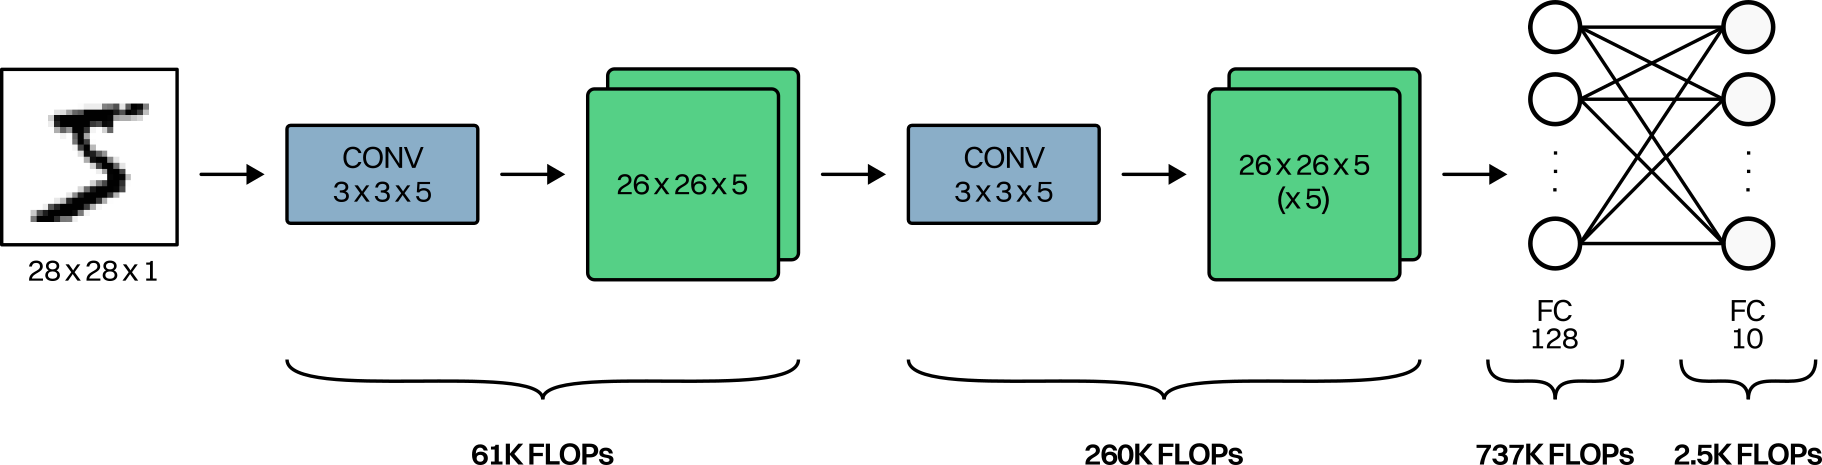
\includegraphics[width=15cm]{images_pfe/mnist.png}
  \caption{Nombre des FLOPs dans le modèle.}
  \label{fig:mnist}
\end{figure}
\FloatBarrier
\medskip

\section{Choix du type d'élagage}
Lors de la conception de notre méthode d'élagage, le choix entre l'élagage structuré et non structuré a été une considération essentielle. L'élagage structuré cible des motifs spécifiques, tels que des neurones entiers, des canaux ou des couches, tandis que l'élagage non structuré élimine des poids individuels sans tenir compte de leur emplacement dans le réseau. Chaque approche offre des avantages distincts et des compromis, influençant leur pertinence pour différentes situations d'élagage. Dans cet section, nous explorons les deux types d'élagage et nous sélectionnons un pour l'utiliser dans notre travail.

L'élagage structurée consiste à supprimer des unités ou blocs entiers du réseau de neurones, tels que des filtres, des canaux (plusieurs filtres) ou des couches entières, tout en conservant l'architecture globale du réseau. Cela permet d'avoir une compression plus importante de notre modèle car des structures entières sont supprimées, ce qui peut conduire à un déploiement très efficace sur des appareils avec des ressources de calculs et de stockage limitées. Cependant, l'élagage structuré peut affecter négativement la précision du réseau puisque certains poids importants peuvent être éliminés, et il pourrait nécessiter un ajustement fin pour récupérer les performances perdues.

D'autre part, l'élagage non structuré permet de supprimer des poids individuels ou des connexions du réseau, ce qui permet potentiellement de mieux conserver la précision. Toutefois, il ne conduit pas toujours à des gains significatifs en termes de mémoire et de temps d'inférence puisque le nombre de calculs reste le même (nous avons le même nombre de filtres et les poids éliminés sont seulement remplacés pare des zéros).

Le choix entre ces deux techniques dépend de facteurs tels que l'architecture spécifique du réseau, le matériel disponible et le compromis souhaité entre la compression et les performances. Dans notre cas, nous souhaitons déployer les modèles élagués dans des appareils avec des ressources limitées, c'est pourquoi d'élagage structuré est la meilleure approche à utiliser. Nous utilisons la norme L1 pour identifier et supprimer les canaux les moins importants. La norme L1 est simplement la somme des valeurs absolues des poids $|w_i|$ du canal (\ref{equ:l1}). Pour chaque canal, la norme L1 des poids du canal est calculée et les canaux avec des valeurs plus faibles sont considérés comme moins importants et sont sélectionnés puis supprimés de la couche de convolution.

\begin{equation}
    L1 Norm = \sum |w_i|
    \label{equ:l1}
\end{equation}

\begin{figure}[hbt!]
  \centering
  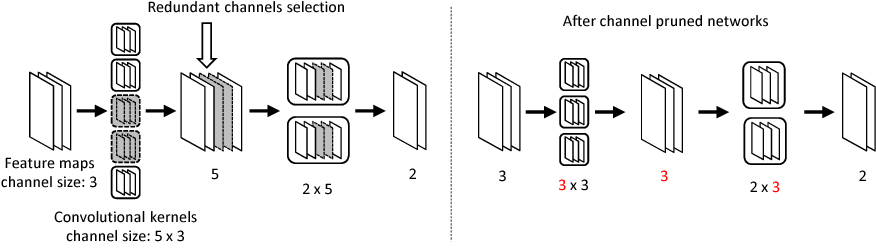
\includegraphics[width=15cm]{images_pfe/channel-pruning.png}
  \caption{Illustration du mécanisme d’élagage des canaux [\cite{Yamamoto2018PCASPC}].}
  \label{fig:mnist}
\end{figure}
\FloatBarrier
\medskip

Après avoir retiré les canaux, le réseau peut subir un ajustement (ré-entraînement) pour rétablir les performances perdues. Cela peut impliquer l'entraînement du réseau élagué, en gardant les valeurs finales des poids après l'élagage, avec un taux d'apprentissage plus petit sur les exemples d'entraînement restants.

\section{Implémentation de l’apprentissage par renforcement}
Comme illustré sur la figure \ref{fig:global-solution}, l'agent reçoit le plongement $s_n$ de la couche $L_n$, puis génère un pourcentage d'élagage de cette couche en tant qu'action $a_n$. Ensuite, La couche $L_n$ est élaguée avec le pourcentage $a_n$ à l'aide de algorithme d'élagage de canaux. Après l'élagage de la couche $L_n$, l'agent passe à la couche suivante $L_{n+1}$ et reçoit son plongement $s_{n+1}$ en entrée. Après avoir élagué toutes les couches, la récompense est évaluée puis renvoyée à l'agent. Dans cette section, nous allons présenter en détail la théorie et l'implémentation de l'algorithme Deep Deterministic Policy Gradient (DDPG) dans notre méthode d'élagage automatique. Nous avons choisi d'utiliser DDPG au lieu de PPO (qui est utilisé dans la méthode présentée par \cite{pfe2022}) parceque DDPG a tendance à converger plus rapidement que PPO dans de nombreux cas. Cette vitesse de convergence est attribuée en partie au fait que DDPG utilise des politiques déterministes et PPO utilise des politiques stochastiques, c'est-à-dire qu'à chaque étape, l'agent DDPG choisit une action spécifique sans aucune composante aléatoire, tandis que l'agent PPO choisit une action avec une composante aléatoire. Cette stochasticité peut ralentir la convergence de l'agent PPO car il doit explorer différentes actions pour déterminer quelle est la meilleure.


\subsection{Agent DDPG}
Dans l'apprentissage par renforcement, les algorithmes de gradient de politique sont utilisés avec une fonction de politique stochastique $\pi(s)$. Cela signifie que, pour un état donné, il y aura une distribution de probabilité pour chaque action dans l’espace d’action. Dans le cas de l'algorithme DDPG (Deep Deterministic Policy Gradient), on utilise une politique déterministe $\mu(s)$ au lieu de la politique stochastique $\pi(s)$. Pour un état \textit{s} donné, il y aura une décision déterministe $\mu(s)$ au lieu d'une distribution sur les actions.

Cet algorithme (DDPG) est un algorithme acteur-critique hors politique (off-policy) qui vise à résoudre des problèmes de contrôle continu, où les actions à prendre sont des valeurs continues plutôt que discrètes. Cet algorithm est une extension de l'apprentissage Q profond et l'algorithme DPG (Deterministic Policy Gradient) qui intègre des réseaux de neurones profonds pour mieux gérer les espaces d'actions et d'états complexes. L'apprentissage Q profond fonctionne dans un espace d'action discret et le DPG l'étend à l'espace d'action continu tout en apprenant une politique déterministe. Donc, Il apprend simultanément une fonction \textit{Q} et une politique déterministe où il utilise des données hors politique et l'équation de Bellman (\ref{equ:bellman}) pour apprendre la fonction \textit{Q}, et puis il utilise la fonction \textit{Q} pour apprendre la politique.

\begin{figure}[hbt!]
  \centering
  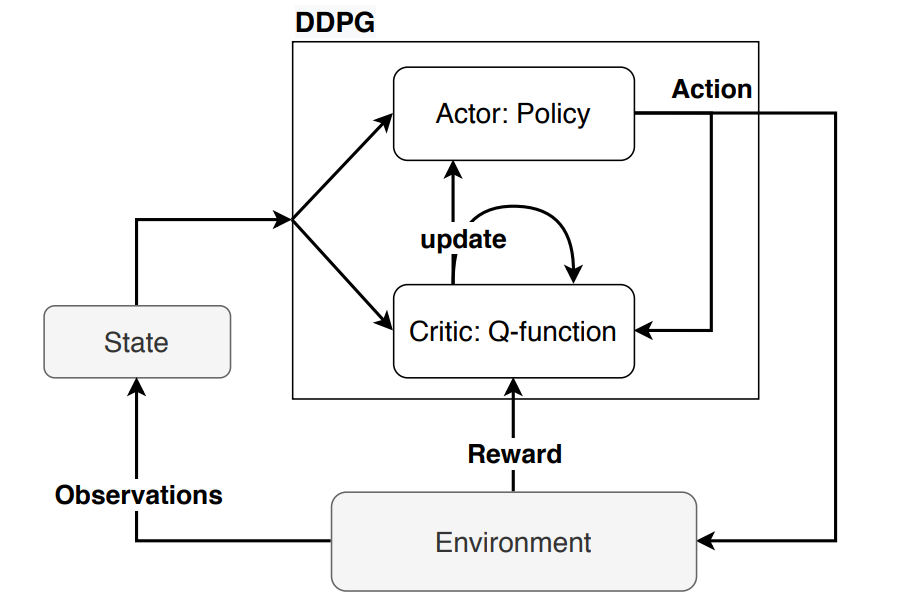
\includegraphics[width=15cm]{images_pfe/ddpg-overview.png}
  \caption{Schéma de présentation de l'algorithme DDPG [\cite{handaoui2020releaser}].}
  \label{fig:ddpg-overview}
\end{figure}
\FloatBarrier
\medskip

L'une des difficultés dans l'apprentissage par renforcement est l'exploration de l'espace d'actions pour découvrir de bonnes stratégies. Dans DDPG, on utilise une politique stochastique pour introduire de l'exploration où on ajoute un bruit additif dans les actions choisies par l'acteur. Dans notre travail, nous utilisons une distribution normale (politique gaussienne) pour le bruit additif (\ref{equ:gaussian-noise}).
\begin{equation}
    \mu^{'} (s_n) \sim N(\mu (s_n | \Theta_{n}^{\mu}), \sigma^2, 0, 1)
    \label{equ:gaussian-noise}
\end{equation}

Pendant l'exploitation, le bruit $\sigma$ est initialisé à 0,5 et diminué de façon exponentielle après chaque épisode. Pour une exploration rapide, nous calculons la récompense sans réglage fin pour avoir une bonne approximation de la précision après le réglage fin.

\subsubsection{Politique gaussienne}
Pour permettre à l'agent de découvrir de nouvelles stratégies potentiellement meilleures, nous allons ajouter du bruit gaussien aux actions choisies par le réseau d'acteur. Ce bruit, également appelé distribution normale ou bruit blanc, est une distribution de probabilité caractérisée par sa moyenne $\mu$ et son écart type $\sigma$. Le bruit ajouté à chaque action est tiré de cette distribution et il permet d'explorer différentes parties de l'espace des actions. La formule \ref{equ:gaussian-distribution} représente la fonction de la distribution gaussienne.
\begin{equation}
    f(x) = \frac{1}{\sigma \sqrt{2\pi}}e^{-\frac{1}{2}(\frac{x-\mu}{\sigma})^2}
    \label{equ:gaussian-distribution}
\end{equation}


Le degré d'exploration peut être contrôlé en ajustant les paramètres de la distribution gaussienne. Nous initialisons l'écart type à une valeur plus élevée (0,5 dans notre cas), ce qui entraîne plus d'exploration, car le bruit ajouté aux actions devient plus important et imprévisible. Après chaque épisode, nous allons diminuer sa valeur de façon exponentielle. Pour la moyenne $\mu$, elle peut être fixée à zéro ou à une petite valeur. Elle n'affecte pas significativement l'exploration, car elle décale le bruit seulement sans altérer son caractère aléatoire.

Ce bruit d'exploration équilibre le compromis entre l'exploration et l'exploitation. Au début, lorsque l'agent apprend, l'exploration est importante pour découvrir différentes actions. À mesure que l'entraînement progresse, le bruit sera progressivement réduit pour se concentrer davantage sur l'exploitation de la politique apprise. Pour ajouter ce bruit aux actions, nous utilisons un générateur de nombres aléatoires pour tirer des échantillons d'une distribution gaussienne

\begin{figure}[hbt!]
  \centering
  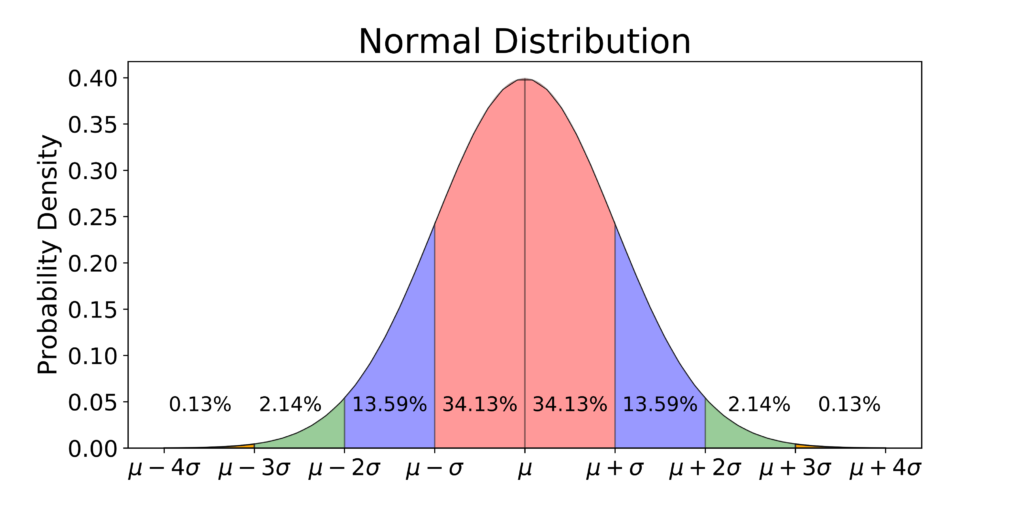
\includegraphics[width=15cm]{images_pfe/normal-distribution.png}
  \caption{Courbe de la distribution gaussienne [\cite{yoseph2019}].}
  \label{fig:normal-distribution}
\end{figure}
\FloatBarrier
\medskip

\subsection{Équations Clés}
\subsubsection{Valeur cible (Target Value) pour le Critique}
Le réseau de critique a pour objectif de minimiser l'écart entre la valeur prédite et la récompense réelle et estimer la récompense cumulative attendue pour une paire état-action donnée. La valeur cible $y_i$ pour le réseau de critique, qui est un élément crucial dans la mise à jour du réseau de critique, est calculée en fonction de la récompense immédiate $r_i$ reçue à l'instant \textit{i} de la valeur estimée de la prochaine paire état-action.
\begin{equation}
    y_i = r_i - b + \gamma \cdot Q(s_{i+1}, \mu (s_{i+1}) | \Theta^Q)
\end{equation}
où $Q(s_{i+1}, \mu (s_{i+1})$ représente la récompense cumulée estimée pour le prochain état $s_{i+1}$ et l'action proposée par le réseau d'acteurs cibles $\mu$, $\gamma$ représente le facteur de remise (discount factor), \textit{b} est la récompense de base et $\mu$ représente le réseau d'acteur cible qui donne l'action suggérée pour le prochain état. La récompense de base \textit{b} est soustraite pour réduire la variance de l'estimation du gradient, qui est une moyenne exponentielle des récompenses précédentes, tandis que le facteur de remise $\gamma$ est fixé à 1 pour éviter de donner la priorité aux récompenses à court terme.

\subsubsection{Mise à jour du Critique}
Le réseau de critique est mis à jour en minimisant la perte moyenne entre la valeur prédite $Q(s_i,a_i)$ et la valeur cible $y_i$. La perte \textit{L} est calculé pour chaque pas de temps, et le but est d'ajuster les paramètres du réseau critique pour minimiser cette perte. 
\begin{equation}
    L = \frac{1}{N}\sum_i(y_i - Q(s_i, a_i | \Theta^Q))^2
\end{equation}
Cette mise à jour aide le réseau critique à mieux se rapprocher de la véritable récompense cumulée attendue.

\subsubsection{Mise à jour de l'Acteur}
L'objectif de l'acteur est d'apprendre une politique qui maximise la récompense cumulée attendue telle qu'estimée par le réseau critique. En d'autres terms, il s'agit de maximiser les valeurs prédites du critique pour les actions prises. La mise à jour du réseau d'acteurs consiste à calculer le gradient de la récompense cumulée attendue par rapport aux paramètres de l'acteur $\Theta_\mu$. Ce gradient est approximé comme suit:
\begin{equation}
    \nabla_{\Theta_\mu}J \approx \mathbb{E}_{s_i}[\nabla_a Q(s_i, a) |_{a=\mu(s_i)} \nabla_{\Theta_\mu}\mu(s_i)]
\end{equation}

où \textit{J} est la fonction d'objectif de l'acteur, $\Theta_\mu$ sont les paramètres du réseau d'acteur, $\mu(s_i)$ est l'action produite par le réseau d'acteur pour l'état $s_i$ et $\nabla_a Q(s_i, a)$ représente le gradient de la valeur du critique par rapport à l'action.


La mise à jour des paramètres $\Theta_\mu$ de l'acteur est effectuée en utilisant ce gradient pour déplacer la politique dans la direction qui augmente la récompense cumulative attendue. La règle de mise à jour des paramètres de l'acteur est donnée par la formule \ref{equ:maj-parameters}.
\begin{equation}
    \Delta \Theta_\mu = \alpha \nabla_{\Theta_\mu}J
    \label{equ:maj-parameters}
\end{equation}
où $\alpha$ est le taux d'apprentissage.

\newcommand\mycommfont[1]{\footnotesize\ttfamily\textcolor{blue}{#1}}
\SetCommentSty{mycommfont}

\subsection{Acteur-Critique}
L'algorithme DDPG utilise deux types de réseaux de neurones profonds: un réseau d'acteur (Actor Network) et un réseau de critique (Critic Network).

\begin{figure}[hbt!]
  \centering
  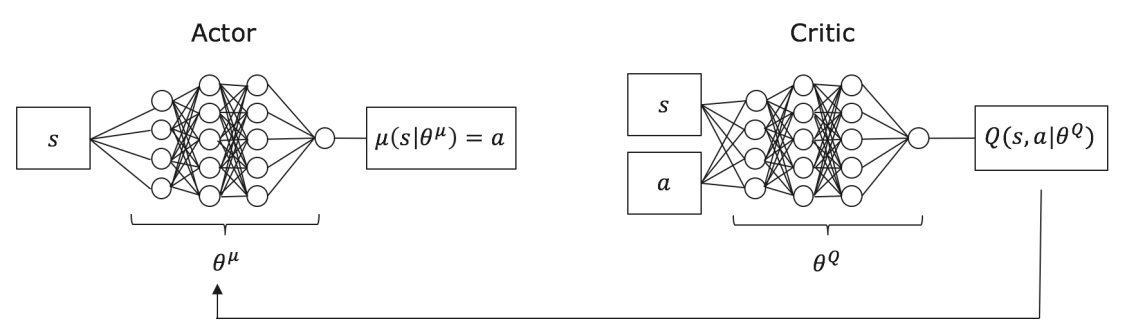
\includegraphics[width=15cm]{images_pfe/ddpg-actor-critic.png}
  \caption{Structure de base de l'agent acteur-critique DDPG. L'acteur prend l'état \textit{s} comme entrée et produit une action basée sur la politique déterministe $\mu$ comme résultat. Le critique prend à la fois l'état et l'action choisie par l'acteur comme entrée et fournit en sortie une valeur \textit{Q} [\cite{Liessner2018DeepRL}].}
  \label{fig:ddpg-actor-critic}
\end{figure}
\FloatBarrier
\medskip

\subsubsection{Réseau d'acteur (Actor Network)}
Le réseau d'acteur est responsable d'apprendre et d'améliorer la politique qui associe des états à des actions continues. Son objectif est de fournir des actions qui maximisent la récompense cumulative attendue sur le temps. Il prend un état actuel $s_i$ (le plongement de la couche \textit{i}) en entrée et génère une action continue $a_i$ (le pourcentage d'élagage de la couche \textit{i}) en sortie qui correspond à l'action que l'agent devrait prendre dans l'état actuel. La caractéristique principale du réseau d'acteur dans l'algorithme DDPG est qu'il apprend une politique déterministe. Pour un état donné, il produit toujours la même action. Ce qui signifie qu'il apprend à produire des actions optimales pour chaque état, ce qui n'est pas le cas pour les politiques stochastiques où l'agent produit une distribution de probabilité sur les actions possibles.

\subsubsection{Réseau de critique (Critic Network)}
Le réseau de critique permet d'approximer la récompense cumulative attendue (aussi appelée fonction de valeur état-action) pour une paire état-action donnée. En d'autres termes, il évalue à quel point une action est bonne dans un état particulier selon la politique actuelle. Il guide le réseau d'acteur en évaluant la qualité des actions choisies. Il prend à la fois un état $s_i$ (le plongement de la couche \textit{i}) et une action $a_i$ (le pourcentage d'élagage de la couche \textit{i}) en entrée et prédit la récompense cumulative attendue $Q(s_i, a_i)$. Cette valeur prédite est fournie au réseau d'acteur pour mettre à jour les paramètres de ce dernier afin d'améliorer la politique, ce qui permet d'obtenir une politique plus performante au fil de l'apprentissage.

\subsection{Protocole de recherche}
Afin de déployer un réseau de neurones très profond sur des appareils avec des ressources matériel limitées, nous devons réduire significativement le nombre de FLOPs et la taille de ce réseau et pour rendre notre méthode plus rapide et plus efficace dans le processus d'élagage, nous allons limiter l’espace d’action de notre agent DDPG, c'est à dire que nous allons limiter le pourcentage d'élagage de chaque couche dans le réseau par la définition d'une borne supérieure $a_{max}$ (on peut prendre $a_{max} = 0.8$). En limitant l'espace d'action, l'agent peut faire une exploration plus efficaces et il peut découvrir des configurations qui optimisent les compromis entre la précision et l'utilisation des ressources.

Pour permettre à l’agent de découvrir de nouvelles stratégies potentiellement meilleures, nous allons ajouter du bruit gaussien aux actions choisies par le réseau d’acteur. Cependant, lors de la mise en œuvre des limites de l'espace des actions pour l'agent DDPG, il est important de veiller à ce que le processus d'exploration de l'agent respecte ces limites. Les stratégies d'exploration telles que l'ajout de bruit aux actions doivent toujours produire des actions dans les bornes spécifiées.

L'algorithme suivant illustre le processus de prédiction du pourcentage d'élagage $a_i$ de la couche $L_i$.



\begin{algorithm}[H]
    \tcc{Initialisation de la taille du modèle élagué}
    \If{\textup{$i$ = 0}}{
        $T_{elague} \gets 0$
    }

    \tcc{Calcul de l'action}
    $a_i \gets \mu^{'}(s_i)$ \;
    \tcc{Limitation de l'action avec le pourcentage d'élagage maximum}
    $a_i \gets min(a_i, a_{max})$ \;

    \tcc{Calcul de la taille du modèle}
    $T_{total} \gets \Sigma_k T_k$ \;
    \tcc{Calcul de la taille des couches suivantes}
    $T_{suivant} \gets \Sigma_{k=i+1} T_k$ \;

    \tcc{Calcul du nombre de paramètres à réduire dans la couche $L_i$ si toutes les couches suivantes sont élaguées avec le pourcentage d'élagage maximal. $\alpha$ représente le pourcentage d'élagage cible du modèle.}
    $T_{cible} \gets \alpha \cdot T_{total} - a_{max}.T_{suivant} - T_{elague}$ \;

    \tcc{Limitation de l'action si elle est trop petite pour atteindre la réduction de taille souhaitée}
    $a_i \gets max(a_i, T_{cible} / T_i)$ \;

    \tcc{Mise à jour de la taille du modèle élagué}
    $T_{elague} \gets T_{elague} + a_i \cdot T_i$ \;

  \Return $a_i$ \;
  \caption{Prédiction du pourcentage d'élagage $a_i$ de la couche $L_i$}
  \label{alg:pruning-ratios}
\end{algorithm}
\FloatBarrier


\subsection{Mémoire de l'agent}
Dans l'algorithme DDPG, l'agent stocke les expériences passées dans une mémoire sous forme de transitions. Chaque transition dans une épisode est de la forme ($s_i$, $a_i$, $R$, $s_{i+1}$), où $s_i$ représente l'état actuel (le plongement de la couche actuelle), $a_i$ et $a_{i+1}$ sont les pourcentages d'élagage de la couche actuelle et la couche suivante respectivement et \textit{R} est la récompense après l'élagage du réseau. L'agent utilise ensuite ces transitions pour mettre à jour les paramètres des réseaux de neurones d'acteur et de critique.

L'utilisation de cette mémoire permet d'améliorer la stabilité de l'apprentissage et la convergence des réseaux en permettant de mélanger les transitions provenant de différentes étapes temporelles afin d'éviter les problèmes de corrélation temporelle, où les transitions consécutives sont fortement liées. De plus, la mémoire permet une meilleure généralisation de l'apprentissage en stockant et en réutilisant des transitions passées. L'agent donc peut acquérir une compréhension plus large de l'environnement et développer des stratégies qui fonctionnent bien dans divers scénarios.

\subsection{Processus d'entraînement de l'agent}
Dans cette section, nous expliquons le processus d'entraînement de l'agent DDPG. Comme illustré dans la figure \ref{fig:ddpg-flow}, ce processus est composé principalement de cinq étapes principales.

\begin{figure}[hbt!]
  \centering
  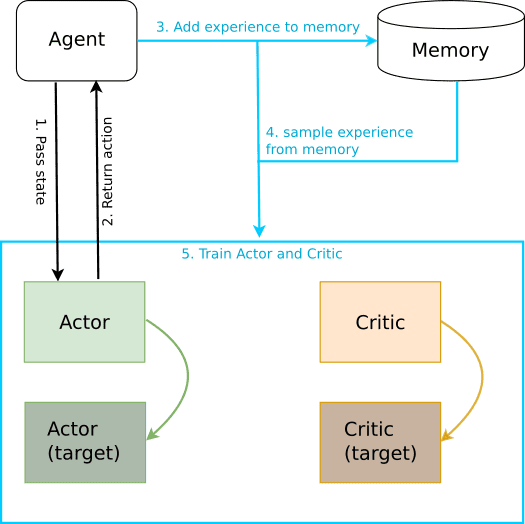
\includegraphics[width=13cm]{images_pfe/ddpgflow.png}
  \caption{Schéma représentant le processus d'entraînement de l'agent DDPG. L'agent est entraîné pour un nombre fixe d'épisodes et, dans chaque épisode, un nombre fixe de pas de temps (timesteps).}
  \label{fig:ddpg-flow}
\end{figure}
\FloatBarrier
\medskip

\begin{enumerate}
    \item \textbf{Passage de l'état à l'acteur}: L'agent reçoit un état $s_i$ de l'environnement, puis il passe cet état au réseau d'acteur ($\mu$). Le réseau d'acteur génère une action $a_i$ en fonction de l'état $s_i$. Cette action est choisie pour maximiser la valeur estimée $Q(s_i, a_i$, qui représente la somme des récompenses futures prévues.
    \item \textbf{Retour de l'action à l'agent}: L'agent reçoit l'action générée $a_i$ du réseau d'acteur, puis il l'envoie à l'environnement. Ce dernier évolue à l'étape \textit{i} et fournit une récompense et un nouvel état $s_{i+1}$ à l'agent.
    \item \textbf{Ajout des expériences à la mémoire}: L'agent crée une expérience en combinant l'état $s_i$, l'action $a_i$, la récompense et le nouvel état $s_{i+1}$ et il l'ajoute à la mémoire.
    \item \textbf{Échantillonnage des expériences de la mémoire}: l'agent échantillonne un lot (batch) d'expériences de la mémoire. Ces expériences échantillonnées forment un ensemble varié de données sur lequel l'agent va apprendre.
    \item \textbf{Entraînement de l'acteur et du critique}: L'agent utilise les expériences échantillonnées dans l'etape précédente pour mettre à jour le réseau de critique (\textit{Q}) en minimisant la différence entre les valeurs prédites et les valeurs cibles basées sur l'équation de Bellman et il calcule le gradient à partir du réseau de critique pour l'utiliser pour mettre à jour le réseau d'acteur ($\mu$). Cette mise à jour du réseau d'acteur vise à maximiser les valeurs \textit{Q} prédites.
\end{enumerate}



\section{Réglage fin après l'élagage}
A la fin de l'exécution de l'algorithme DDPG, nous aurons un modèle élagué qui va avoir une baisse de performance en raison de la perte d'informations qui peut être causée pendant l'élagage puisque nous utilisons l'élagage structuré. On ré-entraîne donc ce modèle afin d'améliorer sa précision pour atteindre une précision proche de celle du modèle original. C'est là qu'interviennent des stratégies clés telles que l'initialisation aléatoire, le rewinding, et le réglage fin (fine-tuning). Ces stratégies sont utilisées pour mettre à jour les paramètres du réseau avant l'entraînement. Dans l'initialisation aléatoire, on affecte des valeurs aléatoires aux paramètres du réseau élagué, tandis que dans le cas du rewiniding, on sauvegarde les paramètres du réseau original avant le premier entraînement pour les utiliser pour initialiser le réseau élagué. Dans le fine tuning, on initialise le réseau élagué par les valeurs des paramètres pré-élagage. La meilleure stratégie pour avoir la plus grande précision est le rewinding, mais elle ne converge pas rapidement [\cite{pfe2022}]. C'est pourquoi nous avons choisi d'utiliser le fine tuning après l'élagage car il permet d'avoir une convergence plus rapide que les deux autres stratégies [\cite{pfe2022}].

Dans cette étape, nous allons ré-entraîner le réseau élagué sur les mêmes données d'entraînement tout en maintenant les poids non supprimés fixés (nous gardons les valeurs des poids résultantes de l'élagage). Cela permet au modèle de réapprendre les relations importantes entre les caractéristiques des données et les étiquettes cibles, en se concentrant sur les parties restantes du réseau. Cependant, nous devons maintenir les poids du réseau qui ont été préservés pendant l'élagage fixés pour garantir que le réseau ne perd pas les connaissances apprises initialement.

Dans notre méthode, nous commençons le ré-entraînement avec un taux d'apprentissage plus faible que celui utilisé dans l'entraînement initial afin d'éviter des mises à jour qui pourraient perturber les poids restants.

\section{Conclusion}
Dans ce chapitre, nous avons présenté les différentes étapes suivies pour concevoir notre propre méthode automatique d'élagage. Nous avons commencé par une vue global de la méthode, où nous l'avons décomposée en quatre étapes principales: \textbf{initialisation}, \textbf{entraînement}, \textbf{élagage} et \textbf{réglage fin}. Dans la partie d'élagage, nous avons utilisé un agent DDPG qui prend en entrée un plongement d'une couche et fournit en sortie le pourcentage d'élagage de cette couche. Après l'élagage, nous avons fait un réglage fin pour améliorer la précision du modèle élagué. Nous aovns également présenté en détails la construction des plongements des couches, les métriques utilisées pour choisir les pourcentages d'élagage, le type d'élagage utilisée (élagage des couches) et l'implémentation de l'algorithme DDPG.

Dans le chapitre suivant, nous allons évaluer et tester notre méthode sur les modèles VGG-19 et ResNet-34. Nous allons présenter d'abord les technologies et outils utilisés pour la conception, puis nous allons comparer les résultats d'élagage de notre méthode avec les résultats d'élagage de quelques méthodes automatique qui effectuent le même type d'élagage que notre méthode (élagage des canaux).






\chapter{Réalisation et tests}
\section{Introduction}
Après avoir exposé en détail notre méthode automatique d'élagage dans le chapitre précèdent, nous discuterons maintenant sur les technologies et outils qui ont été choisis pour matérialiser cette approche et garantir son déploiement efficace. De ce fait, il est essentiel d'examiner en détail les langages de programmation, les bibliothèques et les frameworks qui ont été sélectionnés pour concrétiser notre approche. Nous offrons également un aperçu des stratégies de test que nous avons employées pour évaluer la performance de notre solution. Ces tests ont été établis pour mesurer les performances des modèles VGG-19 et ResNet-34 et la précision de chacun.

\section{Modèles et jeu de données utilisés}
Notre méthode d'élagage a été conçue pour élaguer les réseaux de neurones comportant seulement deux types de couches: les couches de convolution et les couches entièrement connectées. C'est pourquoi nous avons choisi d'utiliser des modèles tels que VGG-19 et ResNet-34. Dans cette section, nous parlerons de l'architecture et de l'organisation de ces deux modèles ainsi que le jeu de données CIFAR-10 qui est utilisé pour les entraîner.
\subsection{CIFAR-10}
CIFAR-10 \footnote{acronyme qui représente le "Canadian Institute for Advanced Research" (Institut canadien de recherches avancées)} est un jeu de données qui est souvent utilisé dans le domaine de la vision par ordinateur. Il se compose d'un total de 60 000 images en couleur de 32x32 pixels chacune, réparties en 10 classes différentes, avec 6 000 images par classe [\cite{krizhevsky2009learning}]. Ces 10 classes d'images comprennent: des avions, des automobiles, des oiseaux, des chats, des cerfs, des chiens, des grenouilles, des chevaux, des bateaux et des camions (\ref{fig:cifar-10-classes}).

\begin{figure}[hbt!]
  \centering
  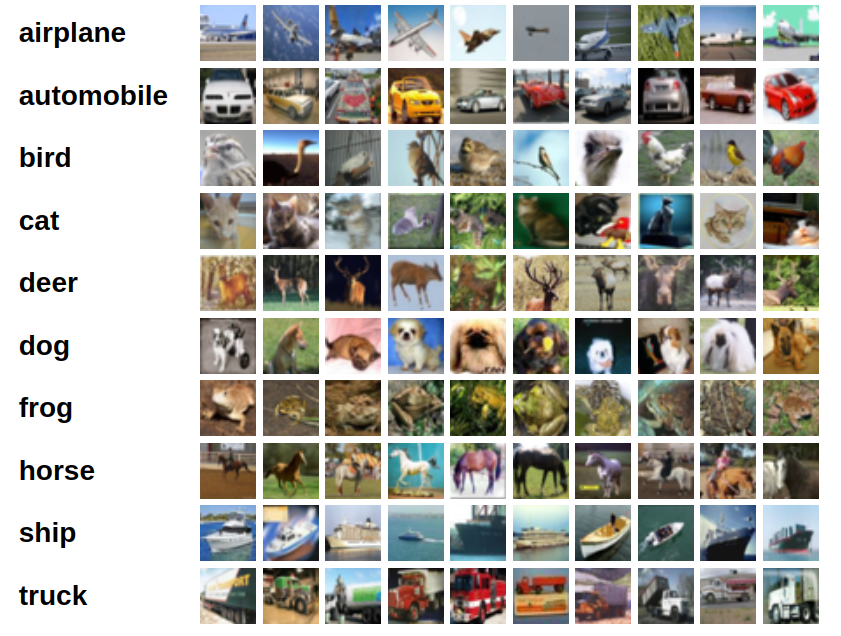
\includegraphics[width=10cm]{images_pfe/cifar-10-classes.png}
  \caption{Les classes du jeu de données CIFAR-10.}
  \label{fig:cifar-10-classes}
\end{figure}
\FloatBarrier
\medskip

Le dataset est divisé en deux ensemble: un ensemble d'entraînement et un ensemble de test. L'ensemble d'entraînement est composé de 50 000 images, tandis que l'ensemble de test est composé de 10 000 images. Dans ce dataset, les images sont de résolution relativement basse et présentent une variabilité dans les poses, l'éclairage, les arrière-plans et les détails, ce qui rend le dataset proche des défis du monde réel. Il est souvent utilisé pour l'entraînement, l'évaluation et la comparaison des performances des algorithmes de classification d'images et des réseaux de neurones convolutionnels (CNN), et il permet de reconnaître leur capacité à généraliser à partir d'un ensemble d'apprentissage limité [\cite{krizhevsky2009learning}].

\subsection{VGG-19}
VGG-19 \footnote{acronyme de "Visual Geometry Group" (famille des modèles développés par l'Université d'Oxford)} est un réseau de neurones convolutif (CNN) très profond qui possède plus de 19,6 milliards de FLOPs et est utilisé fréquemment dans le domaine de la vision par ordinateur. Il est composé de 19 couches, comprenant 16 couches de convolution et 3 couches entièrement connectées, et les images en entrée sont généralement de taille 224x224 pixels. Le réseau commence par des couches de convolutions successives, qui sont suivies de couches de pooling (de type max pooling). Ces dernières permettent de réduire la dimension spatiale de la sortie en ne conservant que les informations les plus importantes [\cite{simonyan2014very}].

Chaque couche de convolution est composée de plusieurs filtres (ou noyaux) 3x3 et un padding (stride) de 1 pour préserver les dimensions. Les filtres possèdent 64, 128, 256, 512 et 512 canaux respectivement. Le nombre de canaux augmente à mesure que l'on progresse dans le réseau. tandis que dans les couches de pooling, on a des fenêtres de 2x2 et un décalage de 2 pour réduire la résolution spatiale [\cite{simonyan2014very}]. 

Une fois que les données sont réduites en termes de dimensions spatiales, elles sont passées à travers plusieurs couches entièrement connectées afin d'effectuer la classification, en associant les caractéristiques apprises aux classes d'objets. La dernière couche de sortie possède le même nombre de neurones que de classes dans le jeu de données. Elle utilise une fonction d'activation softmax pour obtenir des probabilités normalisées pour chaque classe. Dans les couches de convolution, les fonctions d'activation utilisées sont des fonctions ReLU (Rectified Linear Unit) [\cite{simonyan2014very}].

\begin{table}[h!]
\begin{tabularx}{1.0\textwidth} { 
  | >{\centering\arraybackslash}X
  | >{\centering\arraybackslash}X 
  | >{\centering\arraybackslash}X
  | >{\centering\arraybackslash}X
  | >{\centering\arraybackslash}X
  | >{\centering\arraybackslash}X | }
 \hline
 \multicolumn{6}{|c|}{ConvNet Confguration} \\
 \hline
A & A-LRN & B & C & D & E \\
\hline
11 weight layers & 11 weight layers & 13 weight layers & 16 weight layers & 16 weight layers & 19 weight layers \\
\hline
\multicolumn{6}{|c|}{input(224 x 224 RGB image)} \\
\hline
conv 3-64 & conv 3-64 \textbf{LRN} & conv 3-64 \textbf{conv 3-64} & conv 3-64 conv 3-64 & conv 3-64 conv 3-64 & conv 3-64 conv 3-64 \\
\hline
\multicolumn{6}{|c|}{maxpool} \\
\hline
conv 3-128 & conv 3-128 & conv 3-128 \textbf{conv 3-128} & conv 3-128 conv 3-128 & conv 3-128 conv 3-128 & conv 3-128 conv 3-128 \\
\hline
\multicolumn{6}{|c|}{maxpool} \\
\hline
conv 3-256 conv 3-256 & conv 3-256 conv 3-256 & conv 3-256 conv 3-256 & conv 3-256 conv 3-256 \textbf{conv 1-256} & conv 3-256 conv 3-256 \textbf{conv 3-256} & conv 3-256 conv 3-256 conv 3-256 \textbf{conv 3-256} \\
\hline
\multicolumn{6}{|c|}{maxpool} \\
\hline
conv 3-512 conv 3-512 & conv 3-512 conv 3-512 & conv 3-512 conv 3-512 & conv 3-512 conv 3-512 \textbf{conv 1-512} & conv 3-512 conv 3-512 \textbf{conv 3-512} & conv 3-512 conv 3-512 conv 3-512 \textbf{conv 3-512} \\
\hline
\multicolumn{6}{|c|}{maxpool} \\
\hline
conv 3-512 conv 3-512 & conv 3-512 conv 3-512 & conv 3-512 conv 3-512 & conv 3-512 conv 3-512 \textbf{conv 1-512} & conv 3-512 conv 3-512 \textbf{conv 3-512} & conv 3-512 conv 3-512 conv 3-512 \textbf{conv 3-512} \\
\hline
\multicolumn{6}{|c|}{maxpool} \\
\hline
\multicolumn{6}{|c|}{FC-4096} \\
\hline
\multicolumn{6}{|c|}{FC-4096} \\
\hline
\multicolumn{6}{|c|}{FC-1000} \\
\hline
\multicolumn{6}{|c|}{soft-max} \\
\hline
\end{tabularx}
\caption{Les configurations des réseaux VGG (illustrées dans des colonnes selon leurs profondeurs). La colonne E représente la configuration du modèle VGG-19 utilisé [\cite{simonyan2014very}].}
\label{table:vgg-configurations}
\end{table}

\subsection{ResNet-34}
ResNet-34 est un réseau de neurones résiduel profond, composé de 34 couches et possédant plus de 3,6 milliards de FLOPs. Ce type de réseau est caractérisé par l'utilisation de blocs résiduels, en introduisant des connexions résiduelles, également appelées connexions "skip", qui sautent une ou plusieurs couches. Cette caractéristique permet d'exploiter les avantages de la profondeur tout en évitant les problèmes de dégradation de performance qui surviennent lorsque les réseaux deviennent plus profonds [\cite{He_2016_CVPR}].

Le bloc résiduel de base dans ResNet-34 comprend deux couches de convolution 3x3 accompagnées de fonctions d'activation ReLU, et intègre une connexion résiduelle qui agit comme un raccourci autour des couches de convolution, en ajoutant la sortie de la première couche de convolution à la sortie de la deuxième couche. 

\begin{figure}[hbt!]
  \centering
  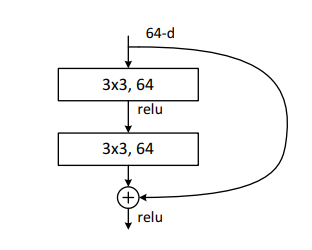
\includegraphics[width=10cm]{images_pfe/residual-bloc.png}
  \caption{Un bloc résiduel de base comme sur la figure \ref{fig:architectures} pour ResNet-34 [\cite{He_2016_CVPR}].}
  \label{fig:residual-bloc}
\end{figure}
\FloatBarrier
\medskip

La fin du réseau ResNet-34 comprend une couche de classification entièrement connectée avec autant de neurones que de classes dans le jeu de données. Une fonction d'activation softmax est généralement utilisée pour obtenir les probabilités de classe normalisées.

\begin{figure}[hbt!]
  \centering
  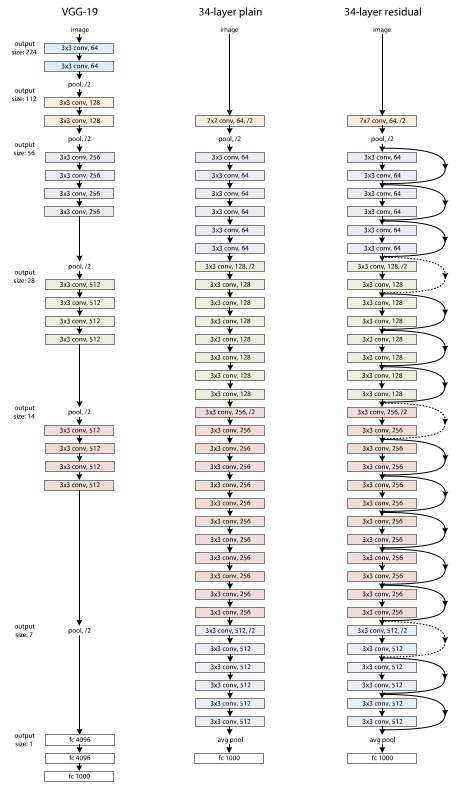
\includegraphics[width=13.5cm]{images_pfe/vgg-19-and-resnet-34.png}
  \caption{Les architectures des modèles utilisés. A gauche: le modèle VGG-19. Au milieu: un réseau simple de 34 couches. À droite: le modèle ResNet-34 [\cite{He_2016_CVPR}].}
  \label{fig:architectures}
\end{figure}
\FloatBarrier
\medskip

\section{Technologies utilisées}
\subsection{Python}

\begin{figure}[hbt!]
  \centering
  
\includegraphics[width=4cm]{images_pfe/python.png}
  \caption{Python.}
  \label{fig:python}
\end{figure}
\FloatBarrier
\medskip

Python joue un rôle important dans le domaine de l'intelligence artificielle (IA) grâce à sa polyvalence, sa simplicité et sa richesse en bibliothèques spécialisées. En tant que langage de programmation, Python est devenu le premier choix  pour de nombreux chercheurs, ingénieurs et développeurs travaillant dans le domaine de l'IA. D'une part, Python est connu pour sa syntaxe claire et lisible, ce qui  permet aux nouveaux arrivants dans le domaine de l'IA de se familiariser rapidement avec les concepts de base. D'autre part, Python offre plusieurs bibliothèques et frameworks spécialisés dans l'IA, tels que TensorFlow, Keras, PyTorch et Scikit-learn. Ces bibliothèques sont souvent utilisées pour le développement de réseaux de neurones, d'algorithmes d'apprentissage automatique et d'autres techniques d'IA. Finalement, Python est un langage polyvalent qui permet aux développeurs de créer et tester différentes approches rapidement.

\section{Bibliothèque utilisées}
Python offre une riche collection de bibliothèques spécialisées dans plusieurs domaines, en particulier l'IA. Ces bibliothèques offrent des outils et des frameworks puissants pour développer des modèles d'apprentissage automatique, des réseaux de neurones, et bien plus encore. Dans cette section, nous allons explorer les bibliothèques que nous avons utilisé pour implémenter et tester notre méthode.
\subsection{NumPy}

\begin{figure}[hbt!]
  \centering
  
\includegraphics[width=4cm]{images_pfe/numpy.png}
  \caption{NumPy.}
  \label{fig:numpy}
\end{figure}
\FloatBarrier
\medskip

NumPy \footnote{acronyme de "Numerical Python"} est une bibliothèque open source qui offre de nombreuses fonctionnalités pour le calcul numérique en Python. Elle offre un support puissant pour la manipulation de tableaux multidimensionnels, ainsi que pour l'exécution de calculs mathématiques complexes sur ces tableaux. Ces tableaux multidimensionnels permettent de stocker et de manipuler efficacement des données numériques sous forme de matrices et de vecteurs. Elle fournit également des fonctions mathématiques de base, des opérations d'algèbre linéaire, des opérations sur les tableaux, des fonctions statistiques et bien plus encore. Elle est largement utilisé en IA pour le traitement et la manipulation de données, la préparation de jeux de données, ainsi que pour la mise en œuvre d'algorithmes d'apprentissage automatique et de réseaux de neurones. La performance élevée de NumPy en calcul numérique en fait un bon choix pour les tâches intensives en termes de calcul.


\subsection{Matplotlib}
\begin{figure}[hbt!]
  \centering
  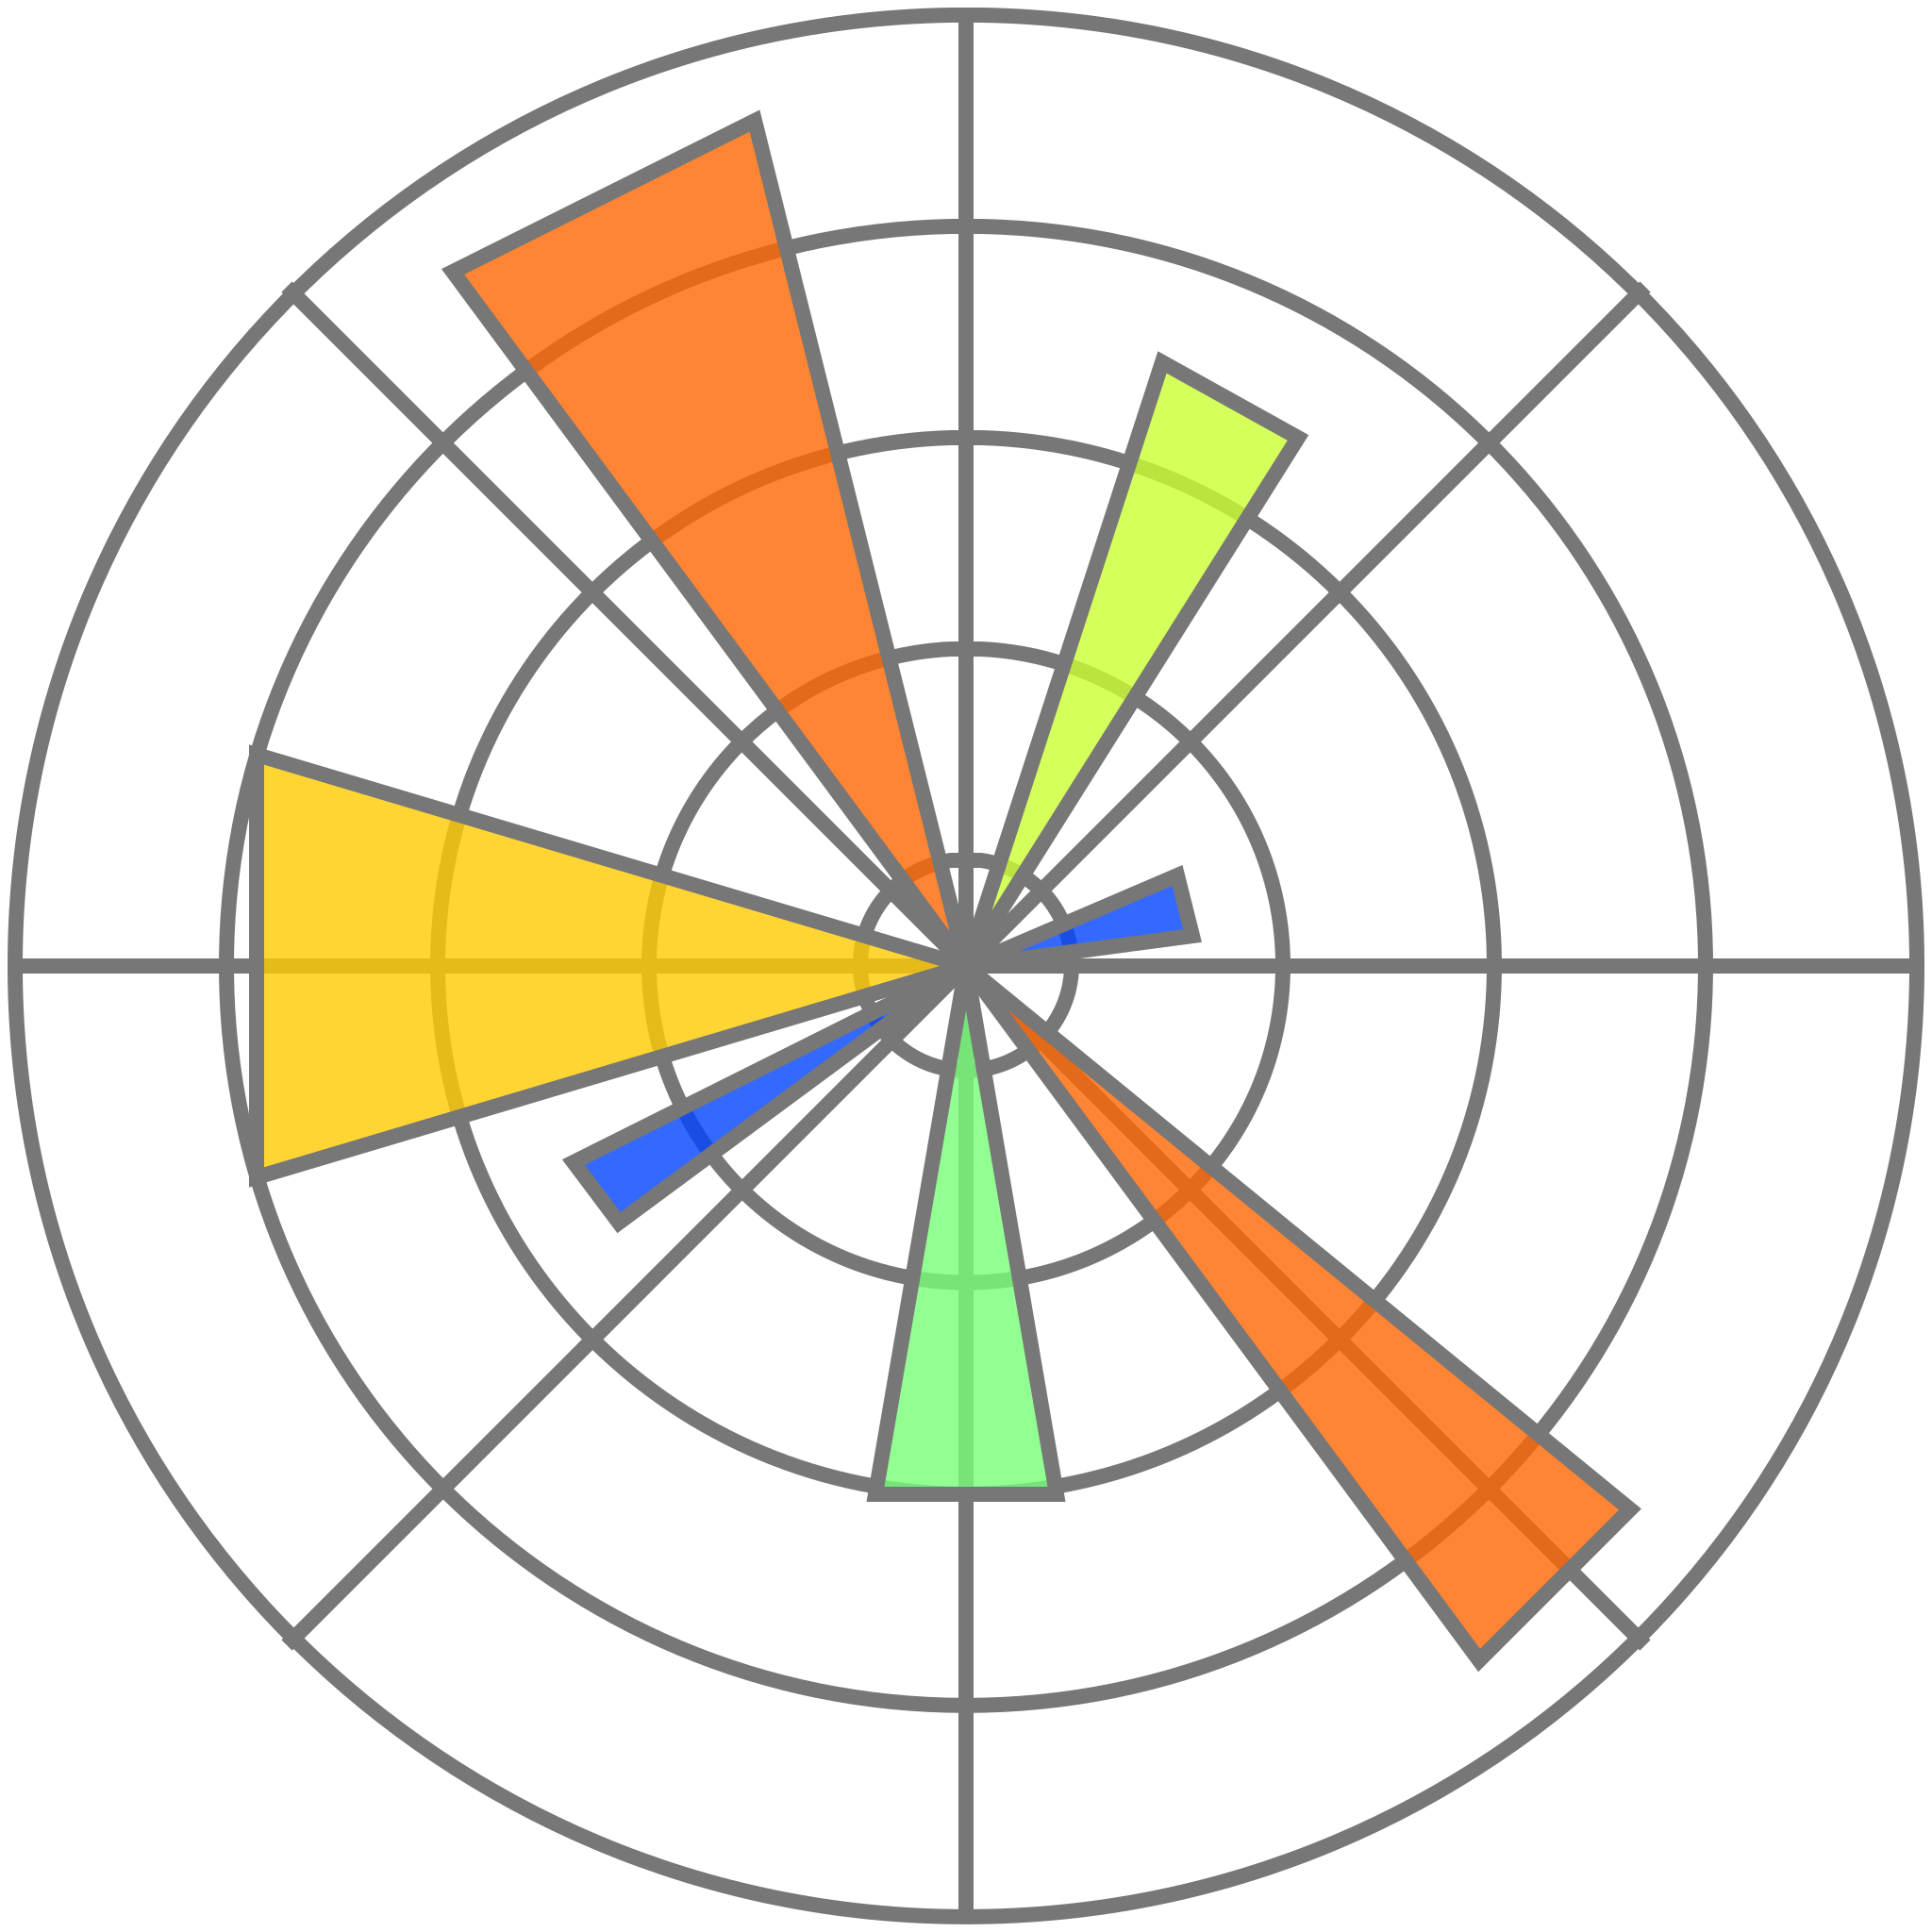
\includegraphics[width=4.5cm]{images_pfe/matplotlib.png}
  \caption{Matplotlib.}
  \label{fig:matplotlib}
\end{figure}
\FloatBarrier
\medskip

Matplotlib est une bibliothèque de visualisation en Python qui aide à créer des graphiques et des visualisations de données de manière interactive et statique. Cette bibliothèque offre un large éventail d'outils pour générer des graphiques de haute qualité à partir de données numériques. Son objectif est de permettre aux utilisateurs de représenter visuellement des données complexes de manière claire et compréhensible. Pour cela, elle propose une grande variété de types de graphiques, tels que les graphiques linéaires, les graphiques en barres, les graphiques à secteurs, les graphiques de dispersion, les graphiques 3D, etc. Elle permet également de personnaliser presque tous les aspects des graphiques, y compris les étiquettes, les couleurs, les styles de ligne, les titres, les axes et les légendes. L'utilisation de Matplotlib est essentielle dans l'analyse de données, la science des données et la recherche en général. En intelligence artificielle et en apprentissage automatique, Matplotlib est souvent employé pour visualiser les performances des modèles, les distributions de données, les tendances, les caractéristiques importantes, les matrices de confusion, les courbes d'apprentissage, etc.

\subsection{Pytorch}

\begin{figure}[hbt!]
  \centering
  
\includegraphics[width=4cm]{images_pfe/pytorch.png}
  \caption{Pytorch.}
  \label{fig:pytorch}
\end{figure}
\FloatBarrier
\medskip

PyTorch est une bibliothèque open-source d'apprentissage automatique et d'intelligence artificielle en Python, développée principalement par Facebook's AI Research lab (FAIR). Elle repose sur un concept fondamental appelé "tenseur", qui est une structure de données multidimensionnelle similaire aux tableaux NumPy et elle est conçue pour faciliter le développement et la mise en œuvre de modèles de réseaux de neurones profonds. PyTorch est surtout distinguée par sa prise en charge des calculs automatiques de gradients, ce qui signifie qu'il est possible de définir des opérations mathématiques sur les tenseurs et que PyTorch peut automatiquement calculer les gradients de ces opérations qui sont nécessaires pour ajuster les poids dans les réseaux de neurones et ainsi minimiser une fonction de perte. Elle est utilisé pour la conception des modèles de réseaux de neurones profonds, y compris les réseaux de neurones convolutionnels (CNN), les réseaux de neurones récurrents (RNN), les transformeurs, etc.

\subsection{Torchvision}

\begin{figure}[hbt!]
  \centering
  
\includegraphics[width=4cm]{images_pfe/torchvision.png}
  \caption{Torchvision.}
  \label{fig:torchvision}
\end{figure}
\FloatBarrier
\medskip

Torchvision est une bibliothèque qui fait partie de PyTorch. Elle est spécifiquement conçue pour faciliter le chargement et la transformation de jeux de données d'images couramment utilisés dans le domaine de l'apprentissage automatique et de la vision par ordinateur. Elle offre des outils pour prétraiter les données d'image, créer des ensembles de données, appliquer des transformations aux images et charger des ensembles de données préexistants. Elle propose des classes pour charger facilement des ensembles de données standard tels que MNIST, CIFAR-10, ImageNet, etc. Elle permet également d'appliquer diverses transformations aux images, telles que le redimensionnement, le recadrage, la normalisation, les rotations, les miroirs, etc. qui sont utiles pour augmenter la variabilité des données.

\subsection{NNI}

\begin{figure}[hbt!]
  \centering
  
\includegraphics[width=6cm]{images_pfe/nni.png}
  \caption{NNI (Neural Network Intelligence).}
  \label{fig:nni}
\end{figure}
\FloatBarrier
\medskip

NNI (Neural Network Intelligence) est une bibliothèque open-source développée par Microsoft Research. Elle fournit un ensemble d'outils et de bibliothèques pour faciliter l'exploration et l'optimisation des espaces d'hyperparamètres, ainsi que pour la recherche automatique d'architectures de modèles. Elle permet aux utilisateurs de définir un espace de recherche pour les hyperparamètres, tels que les taux d'apprentissage, les tailles de lot, les architectures de couches, etc. NNI exécute ensuite des expériences en utilisant différentes configurations d'hyperparamètres et rapporte les résultats, y compris les performances du modèle. Elle est très utile dans le domaine de l'apprentissage automatique, car elle simplifie et automatise le processus d'ajustement des hyperparamètres et d'exploration des architectures, ce qui peut considérablement accélérer le développement de modèles performants.

\section{Outils utilisés}

\subsection{Google Colab}

\begin{figure}[hbt!]
  \centering
  
\includegraphics[width=7cm]{images_pfe/colab.png}
  \caption{Google Colab.}
  \label{fig:colab}
\end{figure}
\FloatBarrier
\medskip

Google Colab (abrégé de Colaboratory) est une plateforme de notebooks interactifs basée sur le cloud, développée par Google. Elle permet aux utilisateurs d'écrire, d'exécuter et de partager du code Python de manière collaborative, sans nécessiter de configuration ou d'installation. Elle propose des notebooks interactifs qui permettent d'insérer des cellules de code exécutable et des cellules de texte et chaque notebook Colab s'exécute dans un environnement virtuel où les utilisateurs peuvent accéder à la puissance de calcul des processeurs graphiques (GPU) et des unités de traitement tensoriel (TPU) pour accélérer l'entraînement de modèles d'apprentissage automatique. Elle propose également de nombreuses bibliothèques préinstallées, mais les utilisateurs peuvent également installer et utiliser des bibliothèques tierces via des commandes simples.

\subsection{Google Drive}

\begin{figure}[hbt!]
  \centering
  
\includegraphics[width=6cm]{images_pfe/drive.png}
  \caption{Google Drive.}
  \label{fig:drive}
\end{figure}
\FloatBarrier
\medskip

Google Drive est un service de stockage en ligne développé par Google pour stocker, synchroniser et partager des fichiers et des dossiers sur le cloud. Il offre une variété de fonctionnalités telles que le stockage en ligne, la synchronisation multi-appareils, le partage de fichiers, la collaboration en temps réel, etc. De plus, il peut être utilisé avec Google Colab.

\section{Tests et résultats}
Cette dernière section présente une analyse des résultats obtenus après avoir tester notre méthode d'élagage. Nous effectuons nos expérimentations sur CIFAR-10 avec deux réseaux profonds classiques: VGG-19 et ResNet-34. Les résultats obtenus sont examinés et comparés avec les résultats des autres méthodes d'élagage, permettant ainsi de dégager des conclusions quant à la performance et l'efficacité de notre méthode. Cette section donc vise à présenter de manière claire et précise les découvertes issues de ces tests.

Le processus d'exécution des tests est décrit comme suit:
\begin{enumerate}
    \item Entraînement du modèle jusqu'à la convergence
    \item Élagage du modèle avec les pourcentages d'élagage fournis par l'agent DDPG
    \item Réglage fin du modèle
    \item Mesure de la précision, la taille, le nombre de paramètres, etc. du modèle élagué
    \item Comparaison du modèle élagué avec le modèle original
\end{enumerate}

On élague les canaux dont les poids ont la plus petite valeur absolue. Le pourcentage d'élagage maximum $a_{max}$ est fixé pour les couches de convolution à 0,8 et pour la couche entièrement connectée à 0,98. Cette limite supérieure $a_{max}$ est utilisée uniquement pour accélérer la recherche. Nous pouvons simplement prendre $a_{max} = 1$ et nous aurons des résultats similaires. Le réseau d’acteurs $\mu$ comporte deux couches cachées, chacune comportant 300 neurones et la couche de sortie finale est une couche sigmoïde pour délimiter les actions dans la plage (0, 1). Le réseau critique \textit{Q} comportait également deux couches cachées, chacune comptant 300 unités. Nous entraînons le réseau avec 64 comme batch size. L'agent DDPG explore d’abord 100 épisodes avec un bruit constant $\sigma = 0.5$, puis exploite 300 épisodes avec un bruit $\sigma$ qui décroît de manière exponentielle.

Pour évaluer la performance de notre méthode, nous l'avons comparée avec les deux méthodes d'élagage citées dans la première partie du rapport: ABCPruner [\cite{lin2020channel}] et CCPrune [\cite{CHEN202135}]. Ces deux méthodes sont des méthodes automatique qui utilisent le même type d'élagage (élagage des canaux). ABCPruner est une méthode basée sur l'algorithme de colonie d'abeilles artificielles (ABC). Dans cette méthode, la recherche du réseau élagué optimal est formulée comme un problème d'optimisation et l'algorithme ABC est utilisé pour le résoudre de manière automatique afin de réduire les interférences humaines. CCPrune (Collaborative Channel Pruning) est une autre méthode qui utilise aussi l'élagage des canaux. Cette méthode introduit d’abord la régularisation sur les poids des couches de convolution et les facteurs d’échelle de la couche BN (Batch Normalization) respectivement, puis elle combine les poids de la couche de convolution et le facteur d’échelle de la couche BN pour évaluer l’importance du canal.

\clearpage

\subsection{VGG-19}
Le tableau suivant représente les résultats après l'application de notre méthode sur VGG-19 avec une comparaison aux deux autres méthodes d'élagage: ABCPruner et CCPrune.

\begin{table}[h!]
\begin{tabular}{|p{3.25cm}|p{3cm}|p{2.25cm}|p{3cm}|p{2.25cm}|}
\hline
Méthode & Précision (\%) & FLOPs (\%) & Paramètres (\%) & Taille (MB) \\
\hline
Modèle original & 93.71 & - & - & 548 \\
\hline
ABCPruner & 93.08 & 73.68 & 88.68 & 62.6 \\
\hline
CCPrune & \textbf{93.78} & 48.92 & 86.82 & 77.2 \\
\hline
Notre méthode & 90.6 & 91.6 & 90.2 & \textbf{52.7} \\
\hline
\end{tabular}
\caption{Résultats d'élagage de VGG-19 sur CIFAR-10. La deuxième colonne indique la précision du modèle. Les troisième et quatrième colonnes indiquent le taux d'élagage des FLOPs et le taux d'élagage des paramètres. La dernière colonne indique la taille du modèle.}
\label{table:vgg-pruning-results}
\end{table}

Les résultats dans le tableau \ref{table:vgg-pruning-results} montrent que les techniques ABCPruner et CCPrune atteignent toujours une précision très proche du réseau original qui est aussi meilleure que celle de notre méthode. Cependant, notre méthode dépasse ces techniques quand nous parlons de la taille du modèle. Nous remarquons qu'avec notre méthode, nous pouvons d'avoir une grande réduction dans la taille du modèle (la taille est 10 fois moins que le modèle original) et dans le nombre de FLOPs et paramètres à cause des pourcentages d'élagage élevés. Cette réduction du nombre de FLOPs signifie que notre méthode effectue moins de calculs que les deux autres méthodes. Nous pouvons donc avoir le meilleur temps d'inférence avec notre méthode. Nous pouvons aussi remarquer que l'utilisation de l'élagage structuré engendre une petite dégradation de la précision des modèles élagués par rapport au modèle original. Cette dégradation est causée par la suppression de canaux entiers, ce qui peut causer une suppression de certains paramètres importants qui peuvent se trouver dans l'un des canaux éliminées.

La figure \ref{fig:vgg-channels} montre les statistiques des canaux restants dans les couche de convolution dans le modèle VGG-19. Sur cette figure, Nous pouvons clairement comprendre la structure du réseau après l'élagage.

Dans VGG-19, 90\% des poids sont dans les couches entièrement connectées. Dans notre méthode, nous avons utilisé l’élagage de canaux entiers en couches de convolution et cela a un effet secondaire intéressant en réduisant également la mémoire. Comme observé dans \cite{molchanov2016pruning}, plus la couche est profonde, plus elle sera élaguée. Cela signifie que la dernière couche de convolution sera beaucoup élaguée et que de nombreux neurones de la couche entièrement connectée qui la suit seront également supprimés.

\begin{figure}[hbt!]
  \centering
  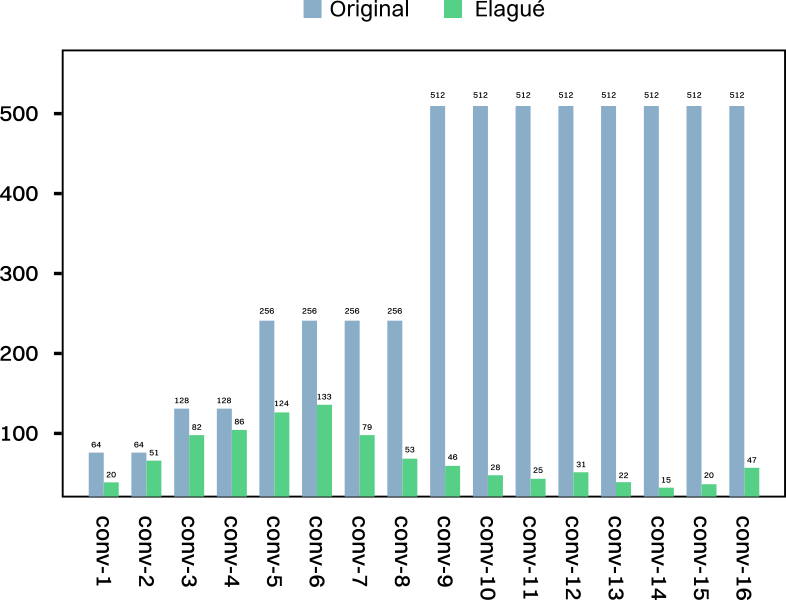
\includegraphics[width=14cm]{images_pfe/vgg-channels.png}
  \caption{Statistiques des canaux restants dans les couches de convolution de VGG-19.}
  \label{fig:vgg-channels}
\end{figure}
\FloatBarrier
\medskip

\subsection{ResNet-34}
Le tableau suivant représente les résultats après l'application de notre méthode sur ResNet-34 et une comparaison avec les deux autres méthodes d'élagage utilisées: ABCPruner et CCPrune.

\begin{table}[h!]
\begin{tabular}{|p{3.25cm}|p{3cm}|p{2.25cm}|p{3cm}|p{2.25cm}|}
\hline
Méthode & Précision (\%) & FLOPs (\%) & Paramètres (\%) & Taille (MB) \\
\hline
Modèle original & 91.45 & - & - & 81.4 \\
\hline
ABCPruner & 89.69 & 58.97 & 51.76 & 39.2 \\
\hline
CCPrune & \textbf{90.76} & 57.55 & 34.78 & 53.0 \\
\hline
Notre méthode & 86.21 & 58.09 & 67.63 & \textbf{26.5} \\
\hline
\end{tabular}
\caption{Résultats d'élagage de ResNet-34 sur CIFAR-10. La deuxième colonne indique la précision du modèle. Les troisième et quatrième colonnes indiquent le taux d'élagage des FLOPs et le taux d'élagage des paramètres. La dernière colonne indique la taille du modèle.}
\label{table:resnet-pruning-results}
\end{table}

Les résultats dans le tableau \ref{table:resnet-pruning-results} sont les même que ceux du modèle
VGG-19. Ils montrent toujours que la précision dans les techniques ABCPruner et CCPrune dépasse la précision dans notre méthode. Cependant, notre méthode dépasse ces deux techniques dans la compression de la taille du modèle et dans le nombre de FLOPs, ce qui nous donnera un meilleur temps d'inférence. Nous remarquons aussi que la taille du modèle élagué avec notre méthode est presque 3 fois moins que le modèle original, ainsi que le nombre de FLOPs et paramètres (les résultats sont résumés dans la figure \ref{fig:resnet-pruning}). Nous avons aussi vu que l'élagage structuré réduit légèrement la précision des modèles élagués par rapport au modèle original et la cause de cette réduction est la même cause mentionnée dans l’interprétation de l’élagage structuré pour le modèle VGG-19.

\begin{figure}[hbt!]
  \centering
  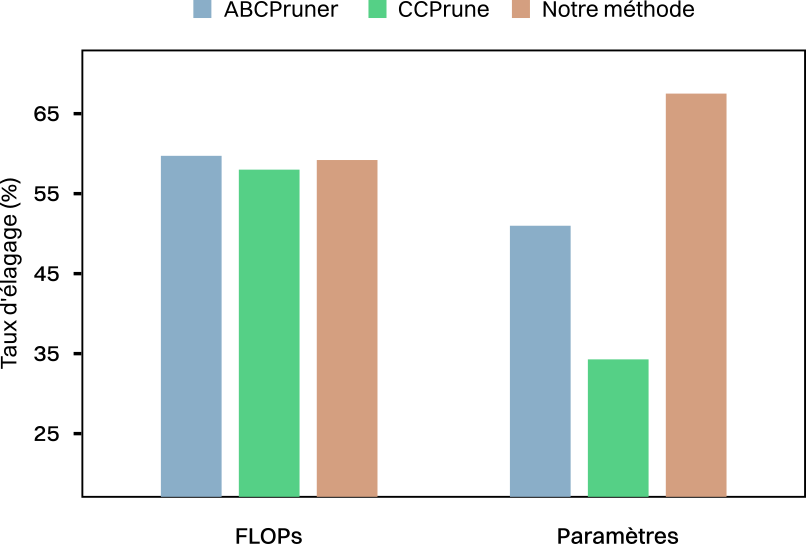
\includegraphics[width=14cm]{images_pfe/resnet-pruning.png}
  \caption{Comparaison entre les taux d'élagage des FLOPs et des paramètres des trois méthodes d'élagage pour le réseau ResNet-34.}
  \label{fig:resnet-pruning}
\end{figure}
\FloatBarrier
\medskip

\section{Conclusion}
En conclusion de ce chapitre dédié aux tests et résultats, l'analyse des résultats d'expérimentations menées sur les modèles VGG-19 et ResNet-34 prouvent l'efficacité de notre méthode d'élagage automatique. Nous avons trouvé que notre méthode permet de réduire significativement la taille des modèles et le nombre de FLOPs, en surpassant les deux méthodes utilisées pour la comparaison (ABCPruner et CCPrune). Ces réductions nous permettent d'avoir de très petits modèles qui sont également très performants et faciles à déployer sur des appareils limités en termes de ressources de calcul et de stockage. Cependant, il est important de souligner que le processus d'élagage n'est pas sans compromis. Les avantages en termes de taille sont parfois accompagnés d'une petite dégradation de la précision qui nécessite de faire un réglage fin après l'élagage afin de restaurer partiellement les performances du modèle initial. De plus, le taux d'élagage optimal peut varier en fonction du même jeu de données et des spécificités de la tâche.

On a également présentée au début du chapitre les modèles utilises pour tester la méthode (VGG-19 et ResNet-34) et le jeu de données utilisé (CIFAR-10) pour l'entraînement de ces modèles, ainsi que les différents technologies et outils utilisés pour la conception de notre méthode. Nous avons utilisé le langage de programmation Python avec plusieurs bibliothèques telles que NumPy, Matplotlib, Pytorch, etc. Ces bibliothèques offrent des outils puissants pour développer et entraîner les différents types de réseaux de neurones.

Enfin, ce chapitre constitue une étape essentielle de ce rapport en fournissant des résultats d'implémentation des concepts et des théories énoncés dans le chapitre précédent. Les résultats obtenus offrent des orientations pratiques pour les applications et les améliorations futures de cette méthode pour élaguer des réseaux de neurones profonds. En considérant ces résultats, la rapport se tourne vers la section finale, où les conclusions et perspectives globales sont tirées.

\chapter*{Conclusion et perspectives}
\addcontentsline{toc}{chapter}{Conclusion et perspectives}
\markboth{Conclusion et perspectives}{Conclusion et perspectives}
\label{chap:conclusion}
%\minitoc

Avec l'augmentation de la profondeur des architecture des réseaux de neurones, le nombre de calculs et la taille des réseaux augmentent également, ce qui rend leurs déploiement sur des appareils dotés d'un matériel limité très difficile et compliqué. L'élagage a émergé comme une approche pour réduire la complexité de ces réseaux profonds. Cependant, cette approche prend beaucoup de temps et nécessite des experts humains afin de bien élaguer un réseau. En raison de ses défauts, des méthodes automatiques utilisant l'apprentissage par renforcement sont apparues. Ces méthodes fournissent des résultats exceptionnels et ont la capacité à s'adapter à une grande variété d'environnements en utilisant des configurations appropriées. Cependant, les algorithmes d'apprentissage par renforcement ne peuvent pas prendre en entrée un réseau profond complet car il est très complexe. Il est donc nécessaire d'utiliser des structures moins complexes comme entrée telles que le plongement de graphe, de chouche, de noeuds, etc. Le plongement est un vecteur unidimentionnel qui garde seulement les informations importantes dans le réseau. En transformant ces données en un vecteur unidimensionnel, cet outil de plongement facilite grandement la capacité de l'agent d'apprentissage par renforcement à appréhender et à interagir avec son environnement.

Dans ce rapport, nous avons découvert les différentes techniques d'élagage des réseaux de neurones, ainsi que les types de plongements et les différents aspects des algorithmes d'apprentissage par renforcement. Nous avons commencé le rapport par une introduction au domaine d'apprentissage profond où nous avons vu quelques définitions et concepts de base, tels que les poids, les connexions, les types de réseaux de neurones, les différents types d'apprentissage (supervisé, non-supervisé, semi-supervisé et par renforcement), etc. Ensuite, nous avons présenté quelques concepts et algorithmes de l'apprentissage par renforcement, tels que les processus de décision de Markov, l'apprentissage Q profond, etc. Nous avons également parlée sur les graphes et les différentes techniques de plongement, ainsi que l'hypothèse du ticket de loterie et les types d'élagage des réseaux de neurones.

On a parlé de tout cela juste pour acquérir suffisamment de connaissances pour pouvoir élaborer une nouvelle approche d'élagage des réseaux de neurones profonds, en utilisant les techniques de plongement de couches et un algorithme d'apprentissage par renforcement complexe pour nous fournir les pourcentage d'élagage du modèle, pour arriver enfin à un modèle de taille considérablement réduite et avec une réduction minimale de la précision. Nous avons commencé par la présentation des modèles testés et le jeux de données utilisée pour les entraîner. Puis, nous avons présenté une vue global de la solution et ensuite les détails de chaque étape de la solution, qui commence par la construction du plongement et finit par le réglage fin. Enfin, nous avons vu les différents résultats d'application de notre méthode sur les modèles et nous les avons comparés avec les résultats de quelques méthodes performantes.

L'avantage le plus important de notre méthode est qu'elle permet de réduire considérablement la taille des modèles et le nombre de calculs, ce qui est idéal pour déployer ces modèles sur des appareils dotés d'un matériel limité. Toutefois, cet avantage est parfois accompagné d'une petite dégradation de la précision, ce qui nécessite de faire un réglage fin après l'élagage afin de restaurer partiellement la précision du modèle initial.

Même si notre méthode donne de très bons résultats, des améliorations sont encore possibles. Nous pouvons apporter ces améliorations à différentes parties de notre processus d’élagage. Par exemple, nous pouvons essayer de généraliser notre méthode à d'autres types d’architectures de réseau autres que les réseaux convolutifs et résiduels. Nous pouvons également modifier l'algorithme d'élagage de l'élagage des canaux vers un autre type d'élagage qui peut contribuer à augmenter la précision de nos modèles. Nous pouvons également essayer de faire d'autres types de plongement, tels que le plongement de l'ensemble du réseau, et utiliser d'autres algorithmes d'apprentissage par renforcement, tels que PPO ou A3C, ou même essayer un algorithme d'optimisation. Nous pouvons aussi essayer de faire l'élagage au début ou pendant l'entraînement afin d'éviter l'étape de réglage fin qui peut prendre du temps pour le ré-entraînement.